\documentclass[UTF8,fontset=none,11pt,a4paper]{ctexrep}

\usepackage[a4paper,top=22mm,bottom=23mm,left=22mm,right=22mm,headheight=15pt]{geometry}
\usepackage{amsmath,amssymb}
\usepackage{graphicx}
\usepackage{booktabs}
\usepackage{longtable}
\usepackage{tabularx}
\usepackage{array}
\usepackage{multirow}
\usepackage{enumitem}
\usepackage{xcolor}
\usepackage{tikz}
\usetikzlibrary{arrows.meta,positioning,fit,calc,shapes.geometric}
\usepackage{listings}
\usepackage{fancyhdr}
\usepackage{hyperref}
\usepackage{caption}
\usepackage{subcaption}
\usepackage{float}

\setCJKmainfont[AutoFakeBold=true]{Microsoft JhengHei}
\setCJKsansfont[AutoFakeBold=true]{Microsoft JhengHei}
\setCJKmonofont[AutoFakeBold=true]{Microsoft JhengHei}

\definecolor{navy}{HTML}{17365D}
\definecolor{blue}{HTML}{2F75B5}
\definecolor{green}{HTML}{548235}
\definecolor{orange}{HTML}{ED7D31}
\definecolor{lightblue}{HTML}{D9EAF7}
\definecolor{lightgreen}{HTML}{E2F0D9}
\definecolor{lightorange}{HTML}{FCE4D6}
\definecolor{codebg}{HTML}{F5F7FA}
\definecolor{darkgray}{HTML}{555555}

\hypersetup{
  colorlinks=true,
  linkcolor=navy,
  urlcolor=blue,
  citecolor=green,
  pdftitle={FPGA3 AES-GCM 175 MHz FPGA Implementation and Verification Report},
  pdfauthor={FPGA3 Project}
}
\graphicspath{{figures/}}
\setlength{\parindent}{2em}
\setlength{\parskip}{0.25em}
\setlist{nosep,leftmargin=2.2em}
\captionsetup{font=small,labelfont=bf}
\renewcommand{\arraystretch}{1.18}

\pagestyle{fancy}
\fancyhf{}
\fancyhead[L]{FPGA3 AES-GCM 175 MHz}
\fancyhead[R]{Implementation and Verification Report}
\fancyfoot[C]{\thepage}

\lstset{
  basicstyle=\ttfamily\small,
  backgroundcolor=\color{codebg},
  frame=single,
  rulecolor=\color{darkgray},
  breaklines=true,
  columns=fullflexible,
  keepspaces=true,
  showstringspaces=false,
  keywordstyle=\color{blue}\bfseries,
  commentstyle=\color{green}
}

\newcommand{\pass}{\textcolor{green}{\textbf{PASS}}}
\newcommand{\fail}{\textcolor{red}{\textbf{FAIL}}}
\newcommand{\code}[1]{\texttt{\detokenize{#1}}}
\newcommand{\hashpair}[2]{\scriptsize\texttt{#1}\newline\texttt{#2}}
\newcommand{\metric}[2]{\textbf{#1}: #2}

\begin{document}

\begin{titlepage}
  \centering
  \vspace*{18mm}
  {\Huge\bfseries\color{navy} FPGA3 AES-GCM IP\par}
  \vspace{4mm}
  {\LARGE 175 MHz FPGA 實作、時序收斂與實板驗證報告\par}
  \vspace{10mm}
  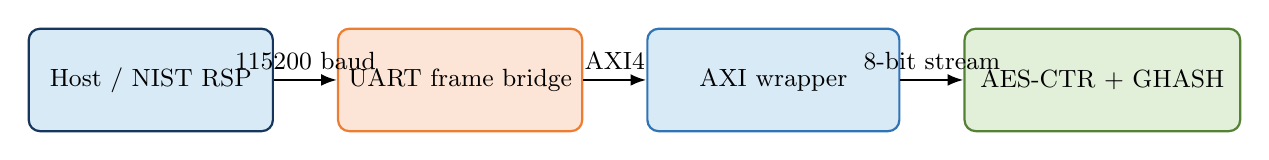
\begin{tikzpicture}[node distance=5mm and 8mm, every node/.style={font=\small}]
    \node[draw=navy,thick,rounded corners,fill=lightblue,minimum width=31mm,minimum height=13mm] (host) {Host / NIST RSP};
    \node[draw=orange,thick,rounded corners,fill=lightorange,right=of host,minimum width=31mm,minimum height=13mm] (uart) {UART frame bridge};
    \node[draw=blue,thick,rounded corners,fill=lightblue,right=of uart,minimum width=32mm,minimum height=13mm] (axi) {AXI wrapper};
    \node[draw=green,thick,rounded corners,fill=lightgreen,right=of axi,minimum width=35mm,minimum height=13mm] (core) {AES-CTR + GHASH};
    \draw[-{Latex[length=2mm]},thick] (host) -- node[above]{115200 baud} (uart);
    \draw[-{Latex[length=2mm]},thick] (uart) -- node[above]{AXI4} (axi);
    \draw[-{Latex[length=2mm]},thick] (axi) -- node[above]{8-bit stream} (core);
  \end{tikzpicture}
  \vspace{12mm}

  \begin{tabular}{rl}
    目標 FPGA： & Digilent Arty A7-100T, XC7A100TCSG324-1 \\
    核心時脈： & 175 MHz（週期 5.714 ns） \\
    工具版本： & Xilinx Vivado 2021.1, build 3247384 \\
    Git branch： & \code{verify/sva-uvm-board} \\
    Build-base commit： & \code{ece78ce9677872d0d20da3b785ab83a48b6a8492} \\
    報告日期： & 2026-08-22 \\
  \end{tabular}

  \vfill
  {\large 結論：175 MHz final strict static audit、六模式 FPGA smoke 與 FPGA NIST 47,250/47,250 均已通過；PartPin 維持 NO。\par}
  \vspace{6mm}
  {\small 本報告所有數值均取自目前工作區 RTL、Vivado DCP/RPT、XSIM log 與 COM4 實板證據；未量測項目會明確標示。\par}
\end{titlepage}

\pagenumbering{roman}
\chapter*{摘要}
\addcontentsline{toc}{chapter}{摘要}

本設計完成一個支援 AES-128、AES-192 與 AES-256 的 AES-GCM authenticated-encryption IP，並以 AXI4-Lite 設定介面、8-bit AXI4-Stream 資料介面與 Arty A7 UART 測試 wrapper 整合。核心以 AES counter mode 產生 keystream，以 GHASH 在 $GF(2^{128})$ 執行驗證；解密 plaintext 在 tag 驗證成功以前不對外釋放，並具備同步 ZEROIZE 與 protocol-abort 清除機制。

最終板級設計在 175 MHz 完成 fresh synthesis、placement、physical optimization 與 routing，並由 immutable routed DCP 進行獨立 v8c strict audit。Routed signoff 為 WNS $+0.029$ ns、TNS $0$、setup failing endpoints $0$、WHS $+0.044$ ns、THS $0$、hold failing endpoints $0$；pulse-width WPWS $+1.607$ ns、TPWS $0$、failing endpoints $0$。17,758 個 routable nets 全部完成 routing，route error 與 DRC violation 均為 0。Methodology Error/Critical Warning 為 0，但有 2 個一般 \code{SYNTH-6 Warning}，因此不宣稱 warning-free。

吞吐率測試以 100 筆、每筆 1024-bit payload 計算：175 MHz 下 AES-128/192/256 加密皆為 1.065398 Gbit/s，解密皆為 1.051705 Gbit/s。v8a bitstream 已經 Vivado Hardware Manager 程式化到 \code{xc7a100t_0}，AES-128/192/256 加解密六模式 smoke 為 6 pass、0 fail。完整 FPGA NIST 在 COM4、115200 baud 執行 47,250/47,250 pass、fail 0、first failure null；47,250-line JSONL 與六個 RSP 來源再經第二位獨立核對通過。UART 實體傳輸仍受 115200 baud 限制，不能把 39.098 cases/s 或 UART 頻寬誤稱為 1 Gbit/s crypto throughput。

\vspace{3mm}
\noindent\colorbox{lightorange}{\parbox{0.95\linewidth}{
\textbf{語音術語對照：}本報告以下採 AES 標準名稱 \emph{SubBytes、ShiftRows、MixColumns、AddRoundKey、Key Expansion}。本設計沒有使用 Edward Lorenz 的 Lorenz chaotic system；若口述的「Edward Lorenz」原意是 \emph{AddRoundKey}，其原理即為 state 與 128-bit round key 的逐位 XOR。
}}

\tableofcontents
\listoffigures
\listoftables
\clearpage
\pagenumbering{arabic}

\chapter{設計範圍與驗證結論}

\section{本報告涵蓋的實體}

本報告同時區分三個層級，避免把核心、wrapper 與板級傳輸混為一談：

\begin{enumerate}
  \item \textbf{AES-GCM 核心：}AES round engines、key expansion、GHASH、descriptor/data queues、authentication 與 ZEROIZE。
  \item \textbf{AXI integration wrapper：}\code{aes_gcm_axi_top.v}，以 AXI4-Lite 控制暫存器與 AXI4-Stream byte interfaces 包裝核心。
  \item \textbf{Arty board test wrapper：}\code{arty_a7_100t_aes_gcm_uart_rsp_top.v}，加入 MMCM、2-stage \code{ASYNC_REG} run-request synchronizer、4-stage synchronous reset-release qualifier、UART RX/TX 與 NIST RSP framing bridge。
\end{enumerate}

\section{最終狀態總表}

\begin{table}[H]
\centering
\caption{最終 FPGA signoff 狀態}
\begin{tabularx}{\linewidth}{>{\bfseries}l l X}
\toprule
項目 & 結果 & 證據 / 說明 \\
\midrule
核心時脈 & 175 MHz & MMCM: $100\times 7/4=175$ MHz；週期 5.714 ns \\
Synthesis & 完成 & v8 fresh build；WNS $-0.298$ ns、TNS $-11.728$ ns、setup FEP 292 \\
Placement + phys\_opt & 完成 & setup WNS $+0.075$ ns；hold WHS $-0.082$ ns、THS $-0.364$ ns、FEP 9 \\
Routing & \pass & audited WNS $+0.029$ ns，WHS $+0.044$ ns，TNS/THS/FEP 全為 0 \\
Pulse width & \pass & WPWS $+1.607$ ns，TPWS $0$，failing endpoints 0 \\
Routing legality & \pass & 17,758/17,758 routable nets fully routed，routing errors 0 \\
DRC / methodology & \pass & DRC violations 0；methodology Error/Critical Warning 0，一般 Warning 2 \\
CDC / reset & \pass & 2 個 CDC-3 safe synchronizers；2-stage request sync + 4-stage release qualifier \\
\code{check_timing} & \pass & 10 個 critical categories 為 0；false-path allowlists 為 input 2 / output 5 \\
Bitstream / config image & \pass & v8c strict-audit \code{.bin} 與 hardware-tested v8a \code{.bin} 完全相同；\code{.bit} header hashes 不同 \\
FPGA programming & \pass & \code{program\_board.tcl} 以 exact v8a \code{.bit} 回報 \code{status=PASS}；device \code{xc7a100t\_0} \\
RTL throughput & \pass & 1.065398 Gbit/s encrypt；1.051705 Gbit/s decrypt \\
FPGA six-mode smoke & \pass & AES-128/192/256 encrypt/decrypt；6/6 pass \\
NIST FPGA test & \pass & 47,250/47,250 pass，fail 0，first failure null；第二位獨立 reconciliation 亦通過 \\
UVM / formal & 部分完成 & XSim UVM 24/0；open-source combinational formal 19/0，不代表 full formal closure \\
PartPin & NO & 無 approved identity-matched production map；未執行 standalone replay \\
\bottomrule
\end{tabularx}
\end{table}

\section{需要正確解讀的限制}

\begin{itemize}
  \item Routed setup margin 為 $+0.029$ ns；若換 Vivado build、constraints、RTL hash 或 implementation directive，必須重跑 signoff。
  \item 0.461 W 為 routed vectorless power estimate，內部 switching activity 信心等級 Medium；它不是電源軌實測值。
  \item 1.05--1.07 Gbit/s 是 RTL/AXI testbench 的 crypto payload throughput。UART 使用 115200 baud，兩者是不同觀測邊界。
  \item Methodology 報告含 2 個 \code{SYNTH-6 Warning}；結果是 Error/Critical-Warning clean，不是 warning-free。
  \item FPGA NIST 47,250 筆已經 exact-bitstream 綁定及兩次 reconciliation 通過；它證明 UART wrapper 的向量正確性，但 39.098 cases/s 仍是 host/UART 交易速率，不是 crypto datapath throughput。
  \item PartPin 尚未完成；full-board route 不能取代 standalone PartPin replay。
\end{itemize}

\chapter{AES 與 GCM 演算法原理}

\section{AES state、key size 與 round 數}

AES 將 128-bit block 視為 $4\times 4$ byte state。初始先做一次 AddRoundKey；中間 round 依序做 SubBytes、ShiftRows、MixColumns、AddRoundKey；final round 省略 MixColumns。Key size 與 round 數如下：

\begin{table}[H]
\centering
\caption{AES key size 與 round 數}
\begin{tabular}{ccc}
\toprule
Key size & $N_k$（32-bit words） & $N_r$（rounds） \\
\midrule
128 bit & 4 & 10 \\
192 bit & 6 & 12 \\
256 bit & 8 & 14 \\
\bottomrule
\end{tabular}
\end{table}

\section{SubBytes：有限體反元素與 affine transform}

SubBytes 是 AES 唯一非線性 round transformation。數學定義為：先在 $GF(2^8)$ 中求 byte 的乘法反元素（0 另行定義），再做 affine transformation；AES 使用不可約多項式
\begin{equation}
  m(x)=x^8+x^4+x^3+x+1.
\end{equation}

目前 RTL 的 \code{sbox.v} 不是在每次運算時計算反元素，而是以完整 256-entry case table 表示 S-box。這是演算法上等價的 lookup-table 方法。實作中：

\begin{itemize}
  \item shared \code{aes_block_engine} 有 16 個 registered S-box，Vivado 將其映射成 8 個 RAMB18；一個 clock 同時處理 state 的 16 bytes。
  \item 兩個 dedicated \code{aes_first_block_engine} 使用 16-way parallel combinational S-box，以 LUT 換取一 round/clock 的短 latency。
  \item key expansion 使用 4 個 registered S-box，映射成另外 2 個 RAMB18。
\end{itemize}

因此板級總計為 10 個 RAMB18。這個選擇保留了 BRAM-based S-box 的規則延遲，也讓 shared engine 的 S-box output 成為顯式 pipeline stage。Reference 資料夾中的 composite-field S-box 文獻說明另一種 area/speed 取捨，但目前 RTL 並未採用 composite-field inversion，不能把該方法誤寫為已實作。

\section{ShiftRows：固定 byte permutation}

ShiftRows 將 state 第 0、1、2、3 列分別循環左移 0、1、2、3 bytes。此操作沒有乘法器或查表，只是 128-bit bus 的固定重新接線。RTL 的 \code{shift\_rows} function 直接重排 bit slices，因此理想上不消耗獨立 arithmetic resources；實際 delay 主要來自 routing 與前後 register/LUT 的組合。

\section{MixColumns：$GF(2^8)$ 固定矩陣乘法}

每一個 4-byte column 乘以下列固定矩陣：
\begin{equation}
\begin{bmatrix}
b'_0\\b'_1\\b'_2\\b'_3
\end{bmatrix}
=
\begin{bmatrix}
02&03&01&01\\
01&02&03&01\\
01&01&02&03\\
03&01&01&02
\end{bmatrix}
\begin{bmatrix}
b_0\\b_1\\b_2\\b_3
\end{bmatrix}_{GF(2^8)}.
\end{equation}

RTL 以 \code{xtime} 實作乘 2：
\begin{equation}
\operatorname{xtime}(a)=(a\ll 1)\oplus
\begin{cases}
\texttt{0x1B}, & a_7=1,\\
0, & a_7=0.
\end{cases}
\end{equation}
乘 3 則為 $\operatorname{xtime}(a)\oplus a$。四個 column 完全平行，只有 shift/XOR/LUT，不使用 DSP。Final AES round 直接選擇 ShiftRows output，繞過 MixColumns。

\section{AddRoundKey：128-bit XOR}

AddRoundKey 為
\begin{equation}
  S_{r+1}=T(S_r)\oplus K_r,
\end{equation}
其中 $T$ 是 SubBytes/ShiftRows/MixColumns 的組合。硬體上是 128 個 parallel XOR。這一層本身不複雜，但 1,920-bit round-key store 的選擇 mux、round-index fanout 與 routing locality 曾是 timing 問題。現在 shared engine 保留四份 4-bit round selector，分別靠近每個 32-bit quarter，避免單一 selector 對 128 個 key bits 的高 fanout。

\section{Key Expansion：RotWord、SubWord、Rcon}

\code{aes_key_context.v} 先擴展並保存最多 15 組 128-bit round keys，共 1,920 bits。每個新 32-bit word 一般為
\begin{equation}
  w_i=w_{i-N_k}\oplus w_{i-1},
\end{equation}
在 $i\bmod N_k=0$ 時，對上一個 word 做 RotWord、SubWord 與 Rcon；AES-256 在 $i\bmod 8=4$ 額外做 SubWord。Rcon 以同一個 $GF(2^8)$ \code{xtime} 更新。

Key expansion 是 iterative FSM，normal word 約 2 clocks，S-box word 約 4 clocks。由 RTL state transition 推得 commit-to-ready latency 為 AES-128 約 100 clocks、AES-192 約 108 clocks、AES-256 約 130 clocks；key ready 後，round keys 由後續所有 records 重用。這能把 key-schedule work 從 steady-state data path 移除，代價是 1,920-bit storage 與前置 key-load latency。

\section{GCM：CTR confidentiality 與 GHASH authentication}

GCM 將 AES counter mode 與 universal hash 結合。先計算
\begin{align}
  H &= E_K(0^{128}),\\
  J_0 &= \begin{cases}
    IV\,\|\,0^{31}\,\|\,1, & |IV|=96,\\
    \operatorname{GHASH}_H(IV), & \text{otherwise},
  \end{cases}\\
  C_i &= P_i\oplus E_K(\operatorname{inc32}(J_0,i)),\\
  T &= \operatorname{MSB}_t\left(\operatorname{GHASH}_H(A,C)\oplus E_K(J_0)\right).
\end{align}

CTR 只需要 AES encryption datapath，解密同樣以 ciphertext XOR keystream 還原 plaintext。GHASH 的 recurrence 為
\begin{equation}
  Y_i=(Y_{i-1}\oplus X_i)\cdot H\quad\text{in }GF(2^{128}),
\end{equation}
field polynomial 為
\begin{equation}
  x^{128}+x^7+x^2+x+1.
\end{equation}

\section{目前 GHASH 的 16-bit digit-serial 架構}

\code{ghash16.v} 每次處理 $X$ 的 16 bits，完成 128-bit multiplication 需要 8 個 digit clocks。Start/load 是獨立 clock，因此外部 initiation interval 為 9 clocks。內部不是串接 16 個 runtime shifts，而是同時建立 $T^0(V)$ 到 $T^{16}(V)$ 的 closed-form linear transforms；依 $X[127:112]$ 選擇 16 個 field terms，再用 balanced XOR tree 做 $16\rightarrow8\rightarrow4\rightarrow2\rightarrow1$ reduction。這將 XOR depth 壓到四層，避免長 XOR chain。

\begin{figure}[H]
\centering
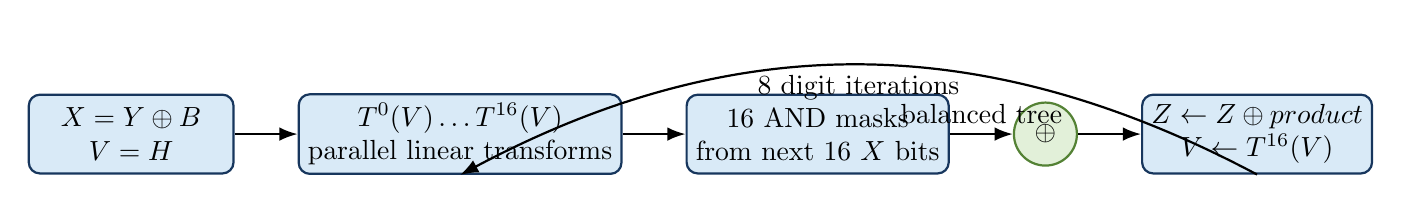
\begin{tikzpicture}[
  block/.style={draw=navy,thick,rounded corners,fill=lightblue,minimum width=26mm,minimum height=10mm,align=center},
  xor/.style={draw=green,thick,circle,fill=lightgreen,minimum size=8mm},
  >=Latex,node distance=7mm and 8mm]
  \node[block] (load) {$X=Y\oplus B$\\$V=H$};
  \node[block,right=of load] (powers) {$T^0(V)\ldots T^{16}(V)$\\parallel linear transforms};
  \node[block,right=of powers] (select) {16 AND masks\\from next 16 $X$ bits};
  \node[xor,right=of select] (xor) {$\oplus$};
  \node[block,right=of xor] (acc) {$Z\leftarrow Z\oplus product$\\$V\leftarrow T^{16}(V)$};
  \draw[->,thick] (load)--(powers);
  \draw[->,thick] (powers)--(select);
  \draw[->,thick] (select)--node[above,sloped]{balanced tree}(xor);
  \draw[->,thick] (xor)--(acc);
  \draw[->,thick,bend right=28] (acc.south) to node[below]{8 digit iterations}(powers.south);
\end{tikzpicture}
\caption{目前 RTL 的 16-bit digit-serial GHASH 資料路徑}
\end{figure}

Reference 文獻中的 Karatsuba-Ofman multiplier、四路 parallel GHASH 與深 pipeline 可達更高吞吐率，但會增加 area、pipeline state 與 verification complexity。目前設計\textbf{沒有使用 Karatsuba}；在 175 MHz 下，GHASH raw block capacity 約為
\begin{equation}
  \frac{128\times175\text{ MHz}}{9}=2.489\text{ Gbit/s},
\end{equation}
已高於 8-bit stream 的理論上限 1.4 Gbit/s，因此現階段不需要以更大 multiplier 換 area。

\chapter{RTL 硬體架構與平行化}

\section{整體資料流}

\begin{figure}[H]
\centering
\resizebox{\linewidth}{!}{%
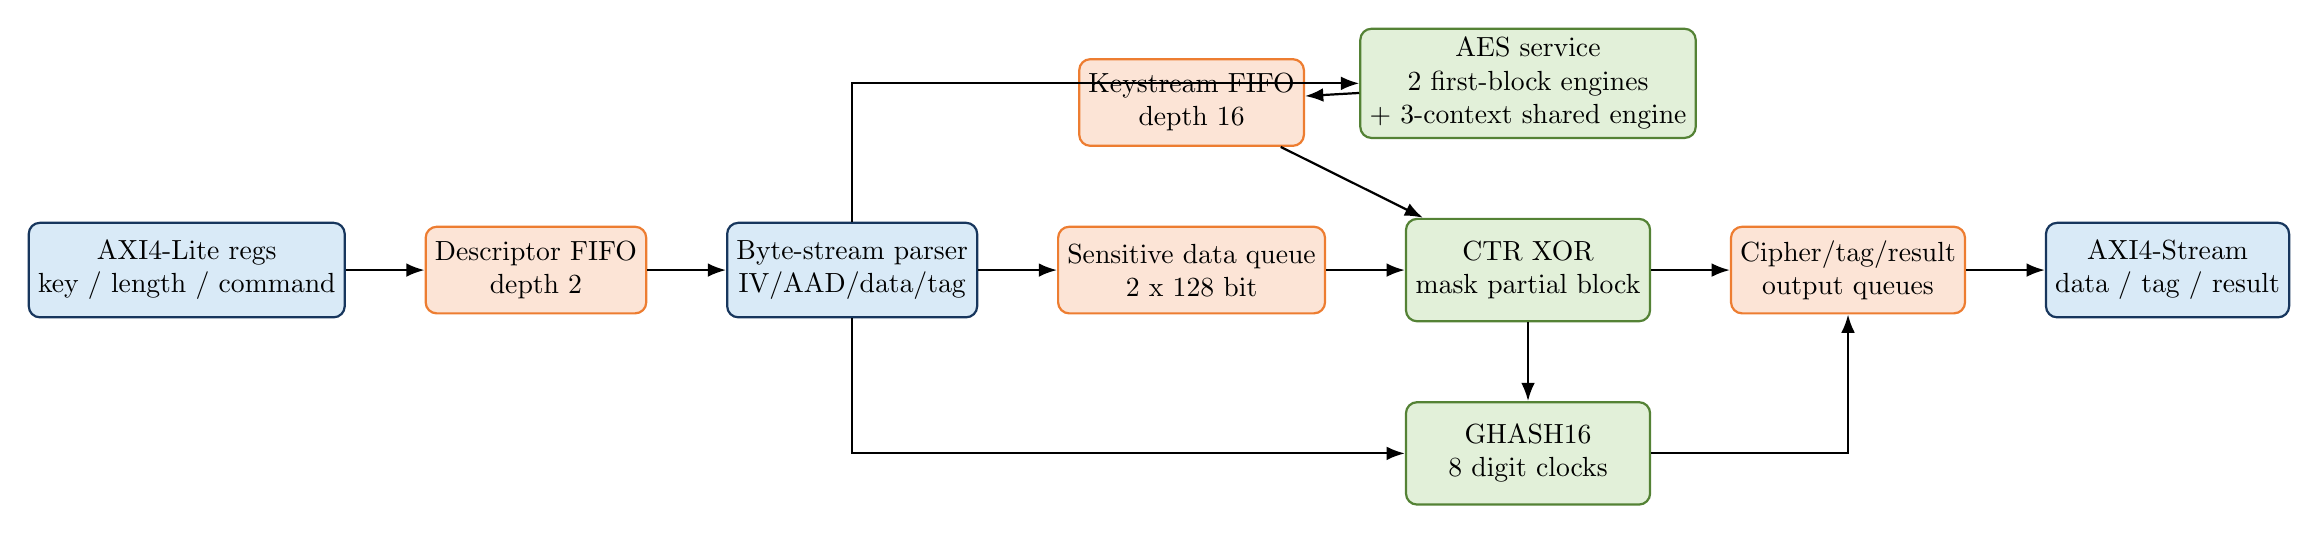
\begin{tikzpicture}[
  block/.style={draw=navy,thick,rounded corners,fill=lightblue,minimum width=29mm,minimum height=12mm,align=center},
  queue/.style={draw=orange,thick,rounded corners,fill=lightorange,minimum width=27mm,minimum height=11mm,align=center},
  crypto/.style={draw=green,thick,rounded corners,fill=lightgreen,minimum width=31mm,minimum height=13mm,align=center},
  >=Latex,node distance=8mm and 10mm]
  \node[block] (regs) {AXI4-Lite regs\\key / length / command};
  \node[queue,right=of regs] (desc) {Descriptor FIFO\\depth 2};
  \node[block,right=of desc] (parser) {Byte-stream parser\\IV/AAD/data/tag};
  \node[queue,right=of parser] (dataq) {Sensitive data queue\\2 x 128 bit};
  \node[crypto,right=of dataq] (xor) {CTR XOR\\mask partial block};
  \node[crypto,above=10mm of xor] (aes) {AES service\\2 first-block engines\\+ 3-context shared engine};
  \node[queue,above=10mm of dataq] (ks) {Keystream FIFO\\depth 16};
  \node[crypto,below=10mm of xor] (gh) {GHASH16\\8 digit clocks};
  \node[queue,right=of xor] (outq) {Cipher/tag/result\\output queues};
  \node[block,right=of outq] (axis) {AXI4-Stream\\data / tag / result};

  \draw[->,thick] (regs)--(desc);
  \draw[->,thick] (desc)--(parser);
  \draw[->,thick] (parser)--(dataq);
  \draw[->,thick] (dataq)--(xor);
  \draw[->,thick] (parser.north) |- (aes.west);
  \draw[->,thick] (aes)--(ks);
  \draw[->,thick] (ks)--(xor);
  \draw[->,thick] (xor)--(outq);
  \draw[->,thick] (xor)--(gh);
  \draw[->,thick] (parser.south) |- (gh.west);
  \draw[->,thick] (gh.east) -| (outq.south);
  \draw[->,thick] (outq)--(axis);
\end{tikzpicture}}
\caption{AES-GCM core 的主要資料流、queues 與 crypto engines}
\end{figure}

\section{AES engines：三 context pipeline 加兩個 first-block engines}

主 \code{aes_block_engine} 以 16 個 registered S-box 共用一條 round datapath，保存三份 state contexts。每個 context 的 round recurrence 為三個 pipeline clocks：

\begin{enumerate}
  \item issue context state 與 round index；
  \item registered S-box output，同時選擇 round key；
  \item ShiftRows / MixColumns / AddRoundKey 回寫 context。
\end{enumerate}

三個 contexts 交錯執行，故 single-request latency 約為 $3N_r$ clocks，但 steady-state completion interval 降為 $N_r$ clocks：AES-128/192/256 分別為 10/12/14 clocks。\code{ready} 具有 finish-now look-ahead，可在 context 完成的同一 edge 接受替代 request。

R55 為了解決 175 MHz 下最前面兩個 CTR blocks 的 first-result latency，新增兩個 \code{aes_first_block_engine}，分別專門處理 block index 0 與 1。每個 engine 一 round/clock，latency 為 10/12/14 clocks。後續 blocks 仍由 shared engine 處理；這不是複製三條完整 AES-GCM lanes，而是針對 startup bubble 的局部平行化。

\begin{table}[H]
\centering
\caption{核心 crypto unit 的 clock latency 與 initiation interval}
\begin{tabularx}{\linewidth}{l c c c X}
\toprule
Unit & AES-128 & AES-192 & AES-256 & 說明 \\
\midrule
Dedicated first-block engine latency & 10 & 12 & 14 & 一 round/clock，兩個 engines 處理 index 0/1 \\
Shared engine nominal single-block latency & 30 & 36 & 42 & 三-stage round recurrence，無其他 context 時 \\
Shared engine steady-state block II & 10 & 12 & 14 & 三 contexts interleaving \\
GHASH latency & \multicolumn{3}{c}{8 digit clocks} & 外部 request II = 9 clocks \\
8-bit stream block transfer & \multicolumn{3}{c}{16 clocks / 128-bit block} & 理論 raw width limit = 1.4 Gbit/s \\
\bottomrule
\end{tabularx}
\end{table}

\section{兩筆 sensitive data queue 與 throughput 改善}

第一個 AES keystream result 的 latency 長於 byte stream 完成第一個 128-bit block 的時間。舊架構會在 block boundary 等待 keystream，造成每筆 record 的 bubble。R55 加入兩筆 128-bit sensitive data queue：input blocks 先排隊，等 ordered keystream FIFO head 到達再 XOR、GHASH 或寫 plaintext bank。Queue 支援同 cycle enqueue/dequeue，並在 protocol abort 或 ZEROIZE 同步清除 plaintext/ciphertext-sensitive payload。

這個改動的重點不是提高 clock frequency，而是提高\textbf{每個 clock 的有效工作比例}：把 first-result latency 與 byte admission overlap。搭配兩個 first-block engines，100 筆 1024-bit records 的 cycles 下降到 encrypt 16,820、decrypt 17,039，三種 key sizes 都超過 1 Gbit/s。

\section{FIFO 與 backpressure}

重要 queue 深度如下：descriptor 2、AES request 4、AES metadata 4、AES result 4、keystream 16、GHASH request 4、ciphertext 4、tag packets 2、authenticated plaintext release 2。所有接口使用 valid/ready；AES engine 本身沒有 output ready，故 result FIFO 吸收完成脈衝。Decrypt plaintext 先存於兩個 packet banks，tag comparison 成功後才進 release queue，避免 unauthenticated plaintext leakage。

\section{ZEROIZE 與 security locality}

過往 timing family analysis 顯示，ZEROIZE/control nets 對 FIFO CE/WE、prep registers 與 round-key controls 的高 fanout/locality 是主要 physical risk。最終 RTL 採用 local registered control、one-hot round-key word write enables、分散的 round selector、同步 reset/zeroize priority 與 queue-local clear。Round48/49/53 security regressions、fast-zeroize、data-buffer clearing 與 NIST simulation suites 均通過。

\chapter{Clock、cycle 與吞吐率}

\section{175 MHz 時脈產生}

Arty A7 板上輸入為 100 MHz。\code{MMCME2\_BASE} 設定 \code{CLKFBOUT\_MULT\_F=7}、\code{CLKOUT0\_DIVIDE\_F=4}，產生 175 MHz core clock：
\begin{equation}
 f_{core}=100\text{ MHz}\times\frac{7}{4}=175\text{ MHz},\qquad
 T_{clk}=\frac{1}{175\text{ MHz}}=5.714\text{ ns}.
\end{equation}
Global clock 使用 1 個 MMCM 與 2 個 BUFG；core clock 有 9,324 個 clock-pin loads，分布於 X0Y2、X1Y2、X0Y3 與 X1Y3 四個 active clock regions。

\section{吞吐率公式與測試定義}

吞吐率必須用 payload bits、測量 clocks 與 clock frequency 同時計算：
\begin{equation}
 \text{Throughput} = \frac{N_{payload\ bits}\cdot f_{clk}}{N_{cycles}}.
\end{equation}
Testbench 每個 mode 執行 100 筆 records，每筆 1024-bit data，故加密為
\begin{equation}
 \frac{100\times1024\times175\times10^6}{16820}
 =1.065398\times10^9\text{ bit/s}.
\end{equation}
解密為
\begin{equation}
 \frac{100\times1024\times175\times10^6}{17039}
 =1.051705\times10^9\text{ bit/s}.
\end{equation}

\begin{figure}[H]
\centering
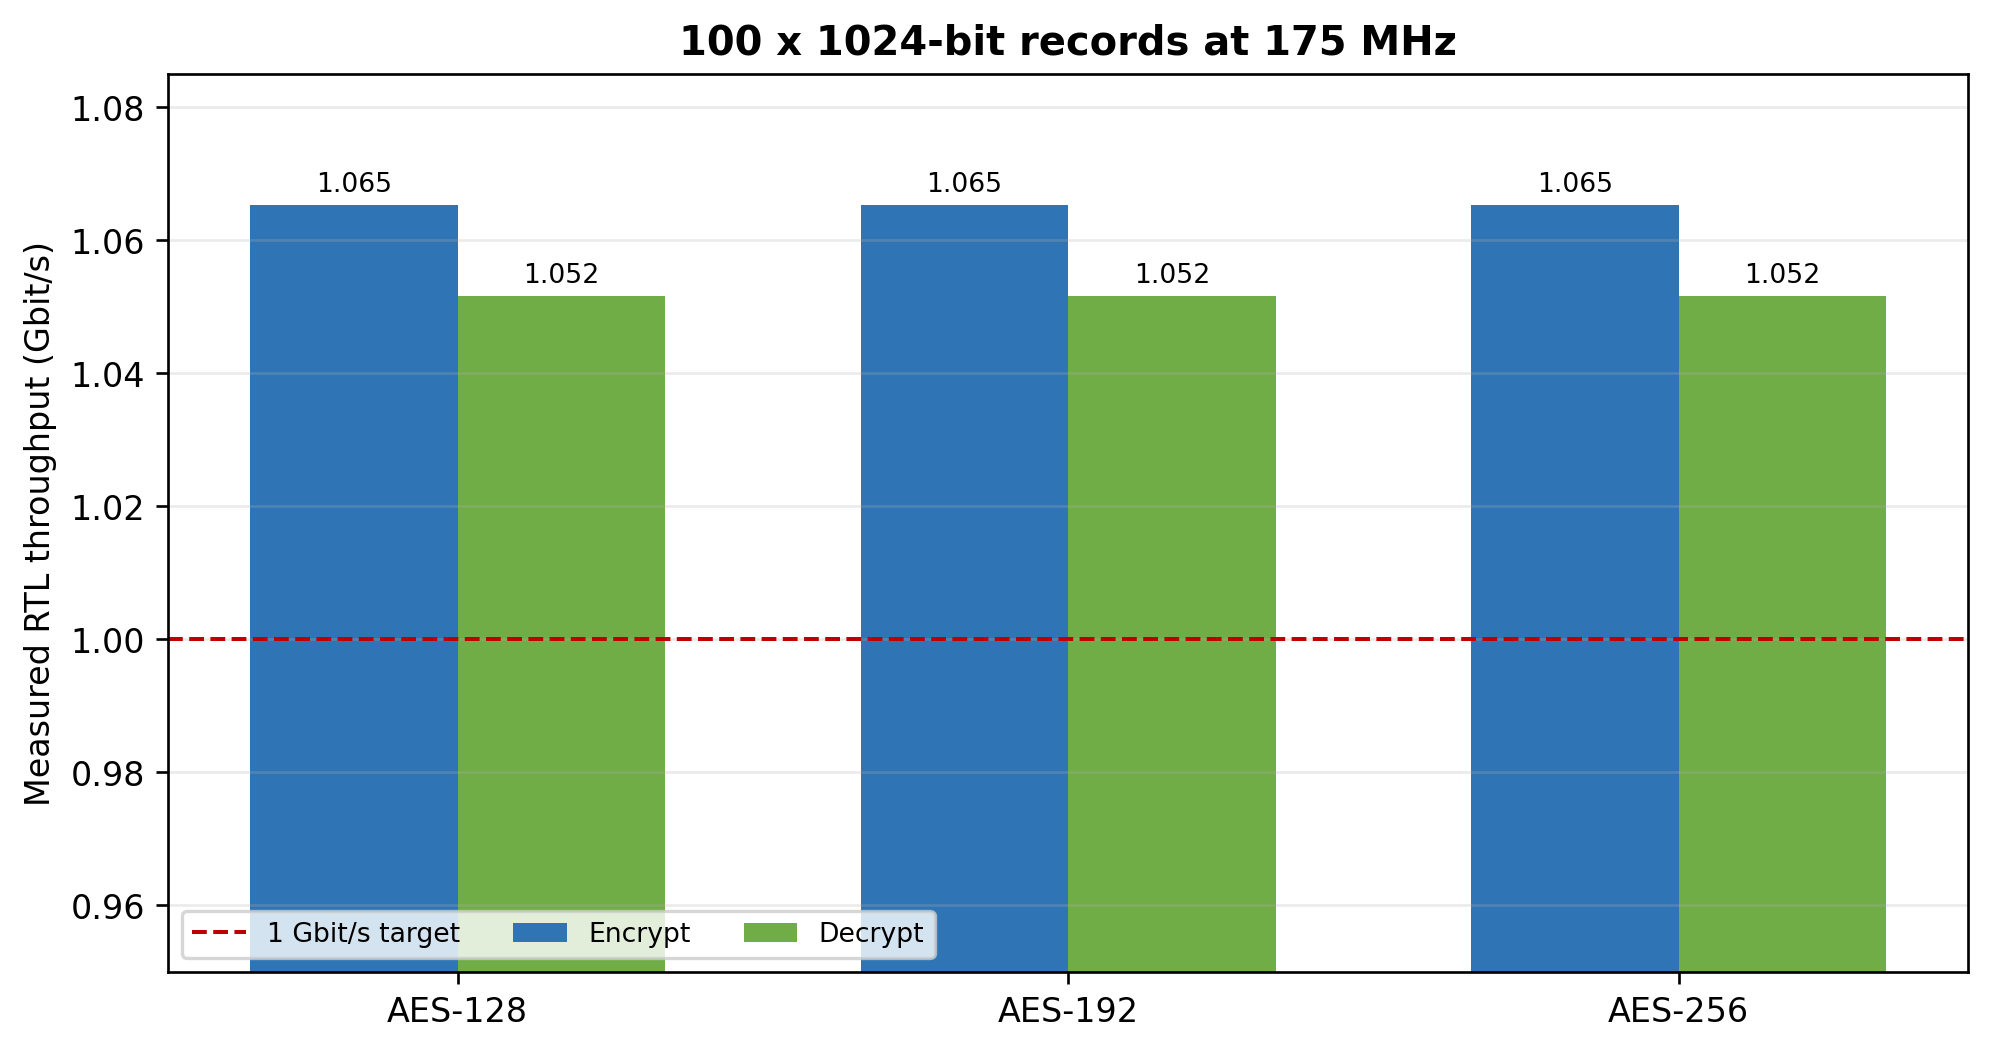
\includegraphics[width=0.88\linewidth]{throughput.png}
\caption{175 MHz 下的六模式 RTL throughput；三種 key size 皆大於 1 Gbit/s}
\end{figure}

Key size 不再改變這個 packet-level measured throughput，是因為最前兩個 blocks 被 dedicated engines 隱藏，後續 shared engine 的 14-clock worst-case II 仍快於 16 clocks/128-bit 的 byte-stream arrival rate。GCM/FIFO/record overhead 使實測值低於 8-bit stream 理論上限 $8\times175=1.4$ Gbit/s。

\section{Latency 與 throughput 的差異}

Latency 是一筆工作從 accept 到 result 的 clocks；throughput 是 steady state 每秒完成多少 payload。Pipeline 可以增加單筆 latency，卻同時降低 initiation interval。例如 shared AES 單筆 nominal latency 可為 30/36/42 clocks，但三 context interleaving 後平均每 10/12/14 clocks 完成一個 block。兩個 first-block engines 則專門縮短 record startup latency。

\section{實板 UART throughput}

板上 NIST wrapper 的 UART 是 115200 baud、8N1。每 8-bit byte 需 10 line bits，因此純 UART payload ceiling 為
\begin{equation}
 115200\times\frac{8}{10}=92.16\text{ kbit/s}.
\end{equation}
每個 frame 還有 command/type 與 16-bit bit-length 共 3 bytes header；例如 128-byte payload 單一 frame 的 wire efficiency 為
\begin{equation}
 \frac{128}{128+3}\times80\%=78.17\%.
\end{equation}
完整 hardware NIST run 共執行 1,208.505 s，平均 39.098 cases/s。這是包含向量長度、frame 數量、host Python、serial turnaround 與 status/data/tag response 的 end-to-end 測試速率，不代表 crypto datapath 的上限。若要在板上直接量測 1 Gbit/s，應改用高速 AXI DMA、Ethernet、PCIe 或純硬體 on-chip counter，不應透過 UART。

\chapter{Synthesis、資源使用率與功率}

\section{Synthesis 的目的}

Synthesis 將 Verilog RTL elaboration 成 technology-mapped netlist，推導 FF、LUT、LUTRAM、BRAM、CARRY、MMCM 等 primitives，並進行 Boolean optimization、memory inference 與初步 timing estimate。它回答「邏輯能否被 FPGA 資源實現、會用多少資源、粗估 critical path」，但\textbf{不能證明實體 timing closure}；真正的 wire delay、placement congestion 與 hold repair 必須在 place/route 後判定。

\section{板級 routed 資源}

\begin{table}[H]
\centering
\caption{Arty A7-100T routed resource utilization}
\begin{tabular}{lrrrr}
\toprule
Resource & Used & Available & Utilization & 說明 \\
\midrule
Total LUT & 12,411 & 63,400 & 19.58\% & 11,333 logic + 1,078 LUTRAM \\
FF & 9,029 & 126,800 & 7.12\% & 包含 core、AXI、UART、reset/heartbeat \\
BRAM36 equivalent & 5 & 135 & 3.70\% & 實體為 10 個 RAMB18 \\
DSP & 0 & 240 & 0.00\% & AES/GHASH 皆用 XOR/LUT/BRAM \\
MMCM & 1 & 6 & 16.67\% & 100 MHz 轉 175 MHz \\
BUFG & 2 & 32 & 6.25\% & core clock 與 MMCM feedback \\
\bottomrule
\end{tabular}
\end{table}

\begin{figure}[H]
\centering
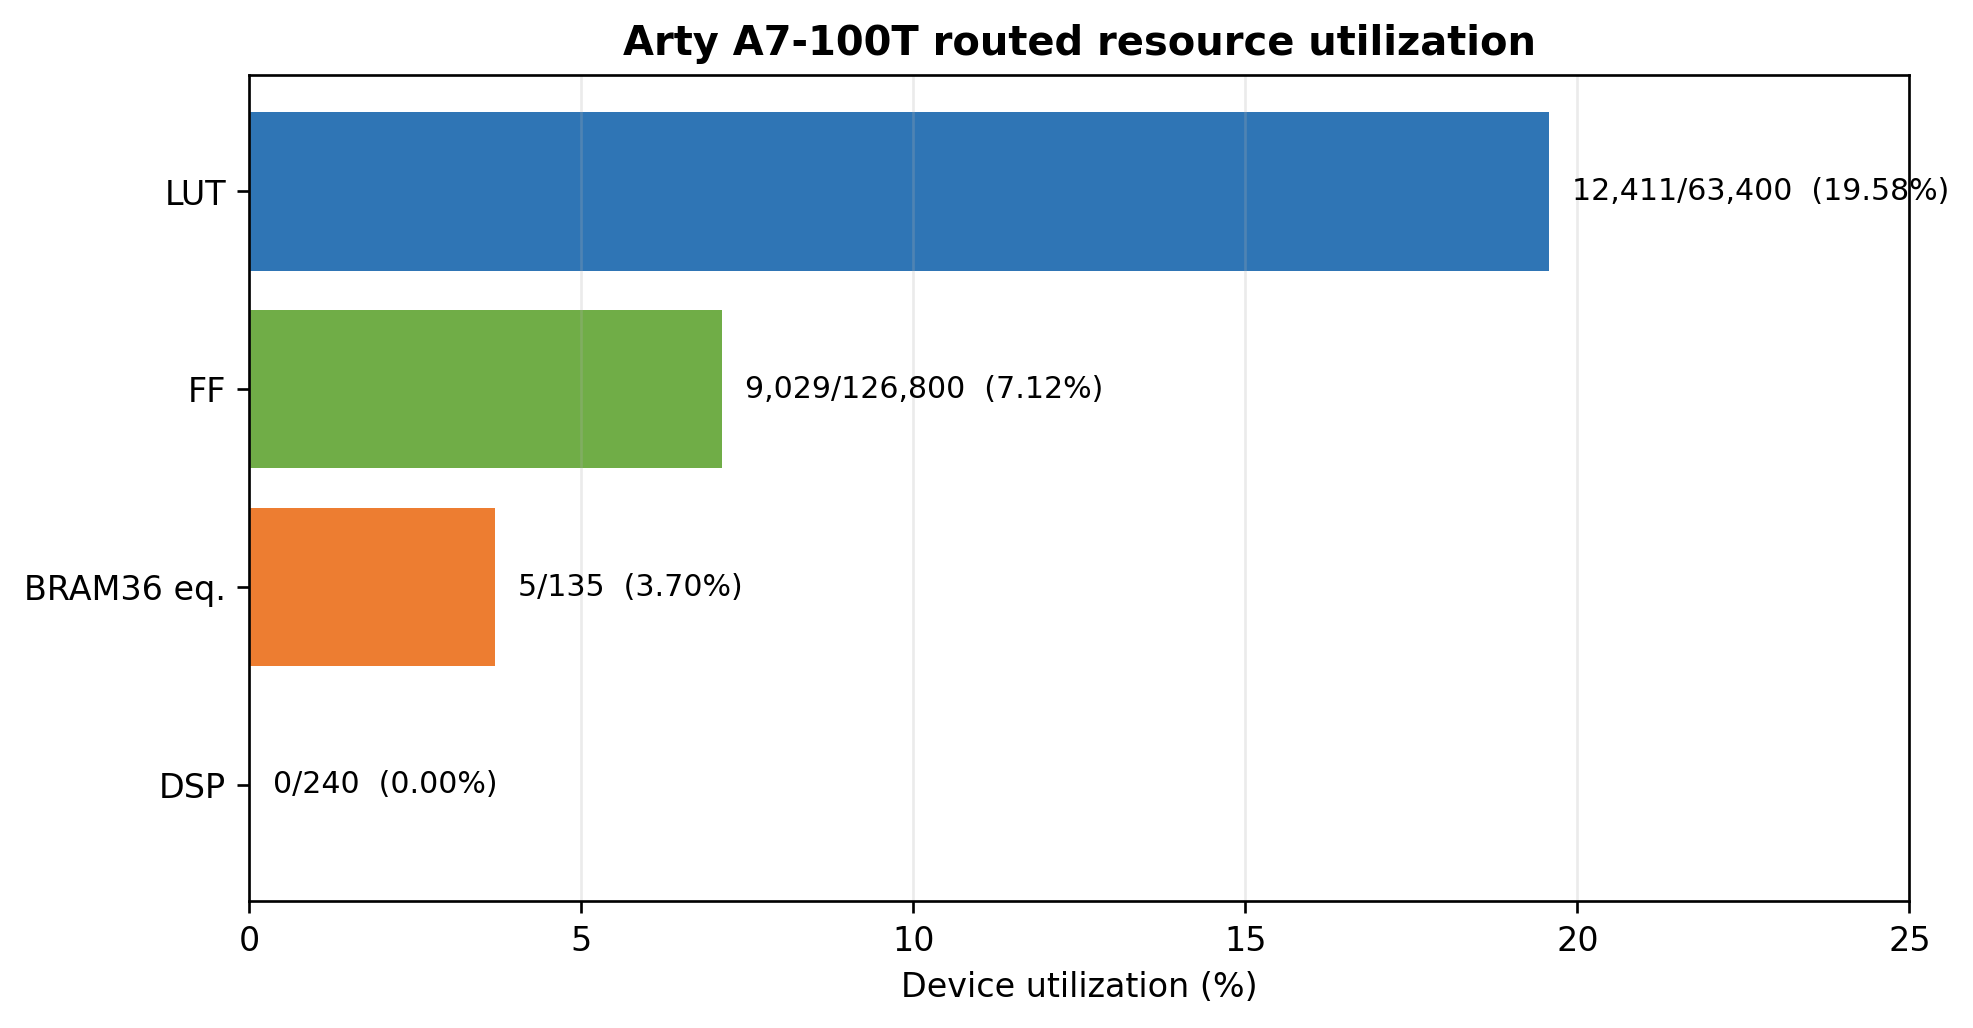
\includegraphics[width=0.88\linewidth]{resource_utilization.png}
\caption{LUT、FF、BRAM 與 DSP 使用率圖；數據來自 final routed DCP}
\end{figure}

\section{主要 hierarchy 資源分布}

\begin{table}[H]
\centering
\caption{Final routed utilization by hierarchy}
\begin{tabular}{lrrrr}
\toprule
Hierarchy & LUT & LUTRAM & FF & RAMB18 \\
\midrule
Board top total & 12,411 & 1,078 & 9,029 & 10 \\
\code{u\_aes\_gcm} & 11,323 & 964 & 8,059 & 10 \\
\code{u\_aes\_gcm/u\_core} & 11,192 & 948 & 7,670 & 10 \\
\code{u\_core/u\_key\_context} & 2,930 & 0 & 2,344 & 2 \\
\code{u\_core/u\_ghash} & 1,442 & 0 & 648 & 0 \\
\code{u\_core/u\_aes\_engine} & 671 & 0 & 719 & 8 \\
\code{u\_core/u\_aes\_first\_engine} & 781 & 0 & 150 & 0 \\
\code{u\_core/u\_aes\_second\_engine} & 783 & 0 & 150 & 0 \\
\code{u\_bridge} & 1,086 & 114 & 694 & 0 \\
\bottomrule
\end{tabular}
\end{table}

\section{使用率降低：UART wide-register arrays 改成 byte memories}

早期 board v3 將最大 1024-bit input/capture payload 實作為大量 FF，並用 dynamic index 寫入。這同時造成 wide mux、reset/control fanout、LUT 與 FF 暴增。v4 將 input、data-capture、tag-capture 改為 8-bit distributed byte memories，保留相同 UART protocol。結果如下：

\begin{table}[H]
\centering
\caption{UART bridge memory refactor 前後資源與 synth timing}
\begin{tabular}{lrrrrr}
\toprule
版本 & LUT & FF & RAMB18 & Synth WNS & Synth FEP \\
\midrule
v3 wide FF arrays & 22,436 & 15,430 & 12 & $-1.192$ ns & 1,489 \\
v4 byte RAM & 12,388 & 8,996 & 10 & $-0.298$ ns & 292 \\
Final v8c strict audit & 12,411 & 9,029 & 10 & $+0.029$ ns & 0 \\
\bottomrule
\end{tabular}
\end{table}

相對 v3，v4 synth 約減少 10,048 LUT（44.8\%）與 6,434 FF（41.7\%）。這是明確的 utilization reduction。它也大幅降低 timing violations；但由於 v3 沒有可比較的 final routed power report，本報告不宣稱精確的功率下降百分比。

\section{Placement 分布與 routing 可視化}

\begin{figure}[H]
\centering
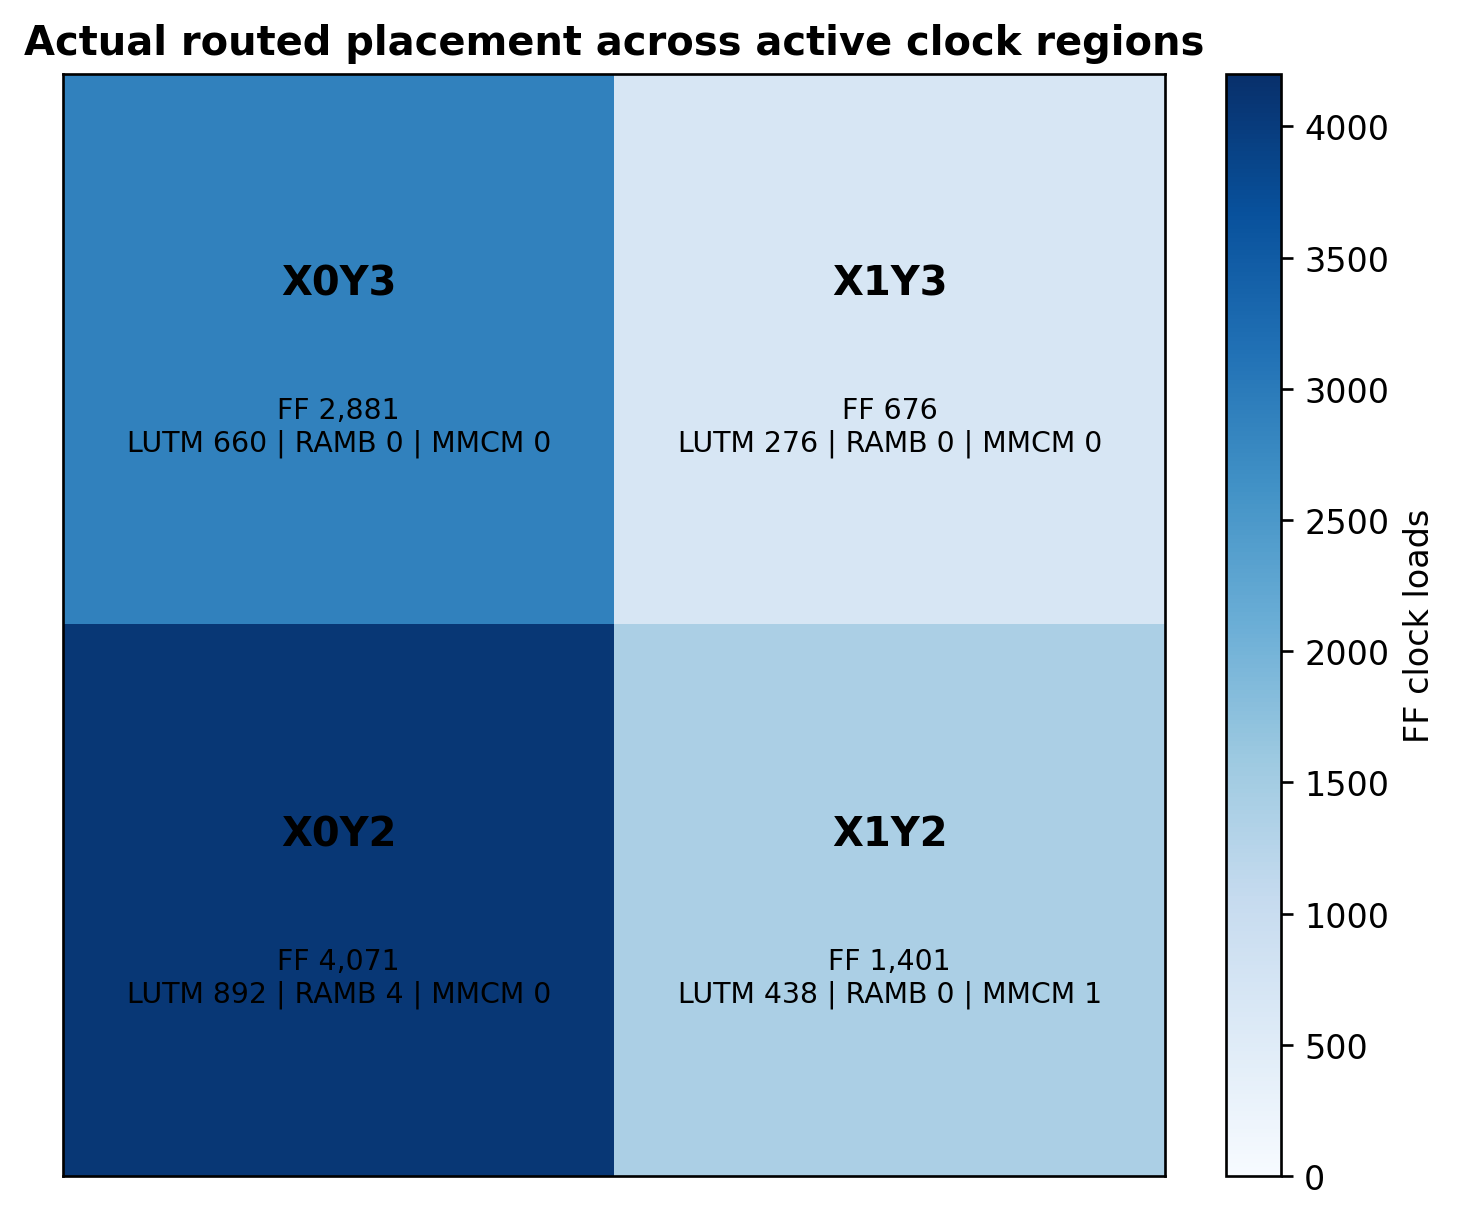
\includegraphics[width=0.78\linewidth]{placement_regions.png}
\caption{Final routed DCP 的 active clock-region placement 摘要。圖中 FF 為該 clock 的實際 clock loads；LUTM/RAMB 欄位取自 Vivado clock-utilization report，並非全器件 primitive 總數。}
\end{figure}

完整 placement 與逐條 routing wire 可在 Vivado 開啟 final routed DCP 後於 Device view 檢查。本報告提供可列印的 clock-region 圖；interactive DCP 才是最完整的「落線圖」來源。Final audit 的 route status 為 17,758 個 routable nets 全部 fully routed、0 routing error。

\section{功率估算}

\begin{table}[H]
\centering
\caption{Vivado routed vectorless power estimate}
\begin{tabular}{lr@{\qquad}lr}
\toprule
項目 & Power & 項目 & Power \\
\midrule
Total on-chip & 0.461 W & Dynamic & 0.363 W \\
Device static & 0.099 W & Junction temperature & 27.1 $^\circ$C \\
Signals & 0.113 W & MMCM & 0.090 W \\
Slice logic & 0.078 W & Clocks & 0.041 W \\
Block RAM & 0.035 W & I/O & 0.005 W \\
\bottomrule
\end{tabular}
\end{table}

\begin{figure}[H]
\centering
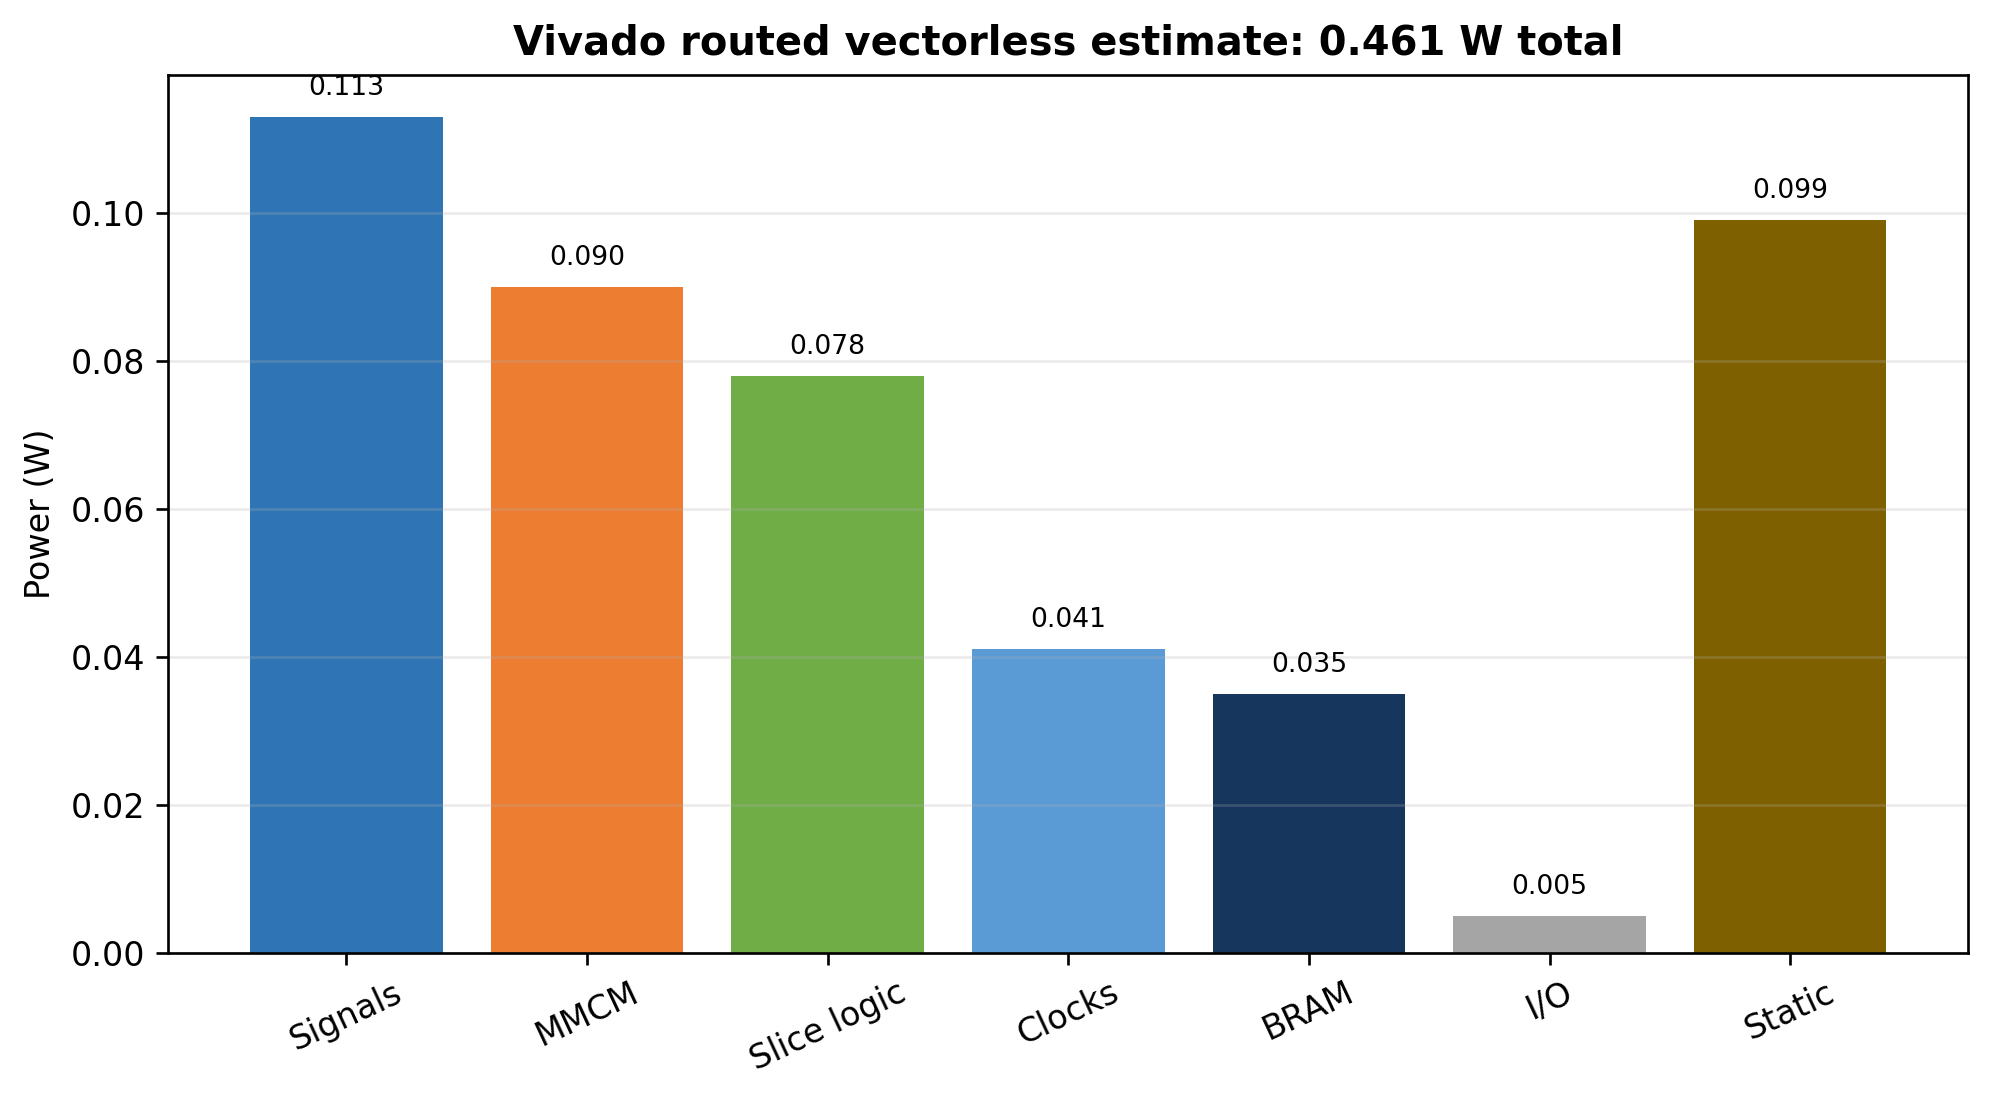
\includegraphics[width=0.86\linewidth]{power_breakdown.png}
\caption{Final routed vectorless power breakdown}
\end{figure}

Power confidence 為 Medium：implementation state 與 clock activity 為 High confidence，但 I/O 與 internal node activity 缺少實際 SAIF/VCD。要得到較可信的 active crypto power，應以代表性 AES-GCM simulation 產生 SAIF，再執行 \code{read\_saif} 與 \code{report\_power}；若要板級實測，需量測 Arty 電源 rail 電流並扣除板上 regulator/USB/LED 等非 IP 功耗。

\chapter{Implementation 與 timing closure}

\section{Vivado flow 與 Tcl 的角色}

Tcl 不是 AES 演算法的一部分，而是 Vivado 的可重現 flow driver。它精確控制 RTL/XDC 載入、synthesis、place、physical optimization、route、reports、DCP hash gate、DRC gate 與 bitstream。使用 Tcl 可以避免 GUI 手動點選造成 directive、constraint 或輸出路徑不一致。

板級 fresh flow 的主要階段為：
\begin{lstlisting}[language=tcl]
synth_design -top arty_a7_100t_aes_gcm_uart_rsp_top \
             -part xc7a100tcsg324-1
opt_design -directive ExploreWithRemap
place_design -directive ExtraNetDelay_high
phys_opt_design -directive AggressiveExplore  # pre-route
route_design -directive Explore
phys_opt_design -directive AggressiveExplore  # post-route
report_timing_summary
report_utilization -hierarchical
report_route_status
report_drc
report_methodology
report_cdc -details
check_timing -verbose
write_checkpoint
write_bitstream
\end{lstlisting}

v8 是 fresh synthesis/place/route，沒有重用舊 placed/routed checkpoint。完成後，\code{audit\_routed\_board.tcl} 以預期 SHA-256 開啟 immutable routed DCP，在獨立的 \code{resetqual4\_audit\_v8c} 目錄重新產生 timing、pulse-width、route、DRC、methodology、CDC、\code{check\_timing}、utilization、clock 與 power 證據，並輸出 bit/bin。Audit script SHA-256 為 \code{62C653E5E49723A51726B92B0D475BA11C55F24A3648D59359A2ABCE99C9286E}；輸入 routed DCP SHA-256 為 \code{A91758ED87EB56648EEF0CAB67B2C50D198D00A2D5088E624B507687D99C016B}。

中間的 v8b 結果因 audit gate 實作誤判而被拒絕；這是 gate logic 的 false rejection，不是 routed DCP 的 timing 或 legality fault。修正 gate 後，v8c 對同一個 hash-matched routed DCP 完成 strict audit 並通過所有 hard gates。

\section{Timing iteration 結果}

\begin{figure}[H]
\centering
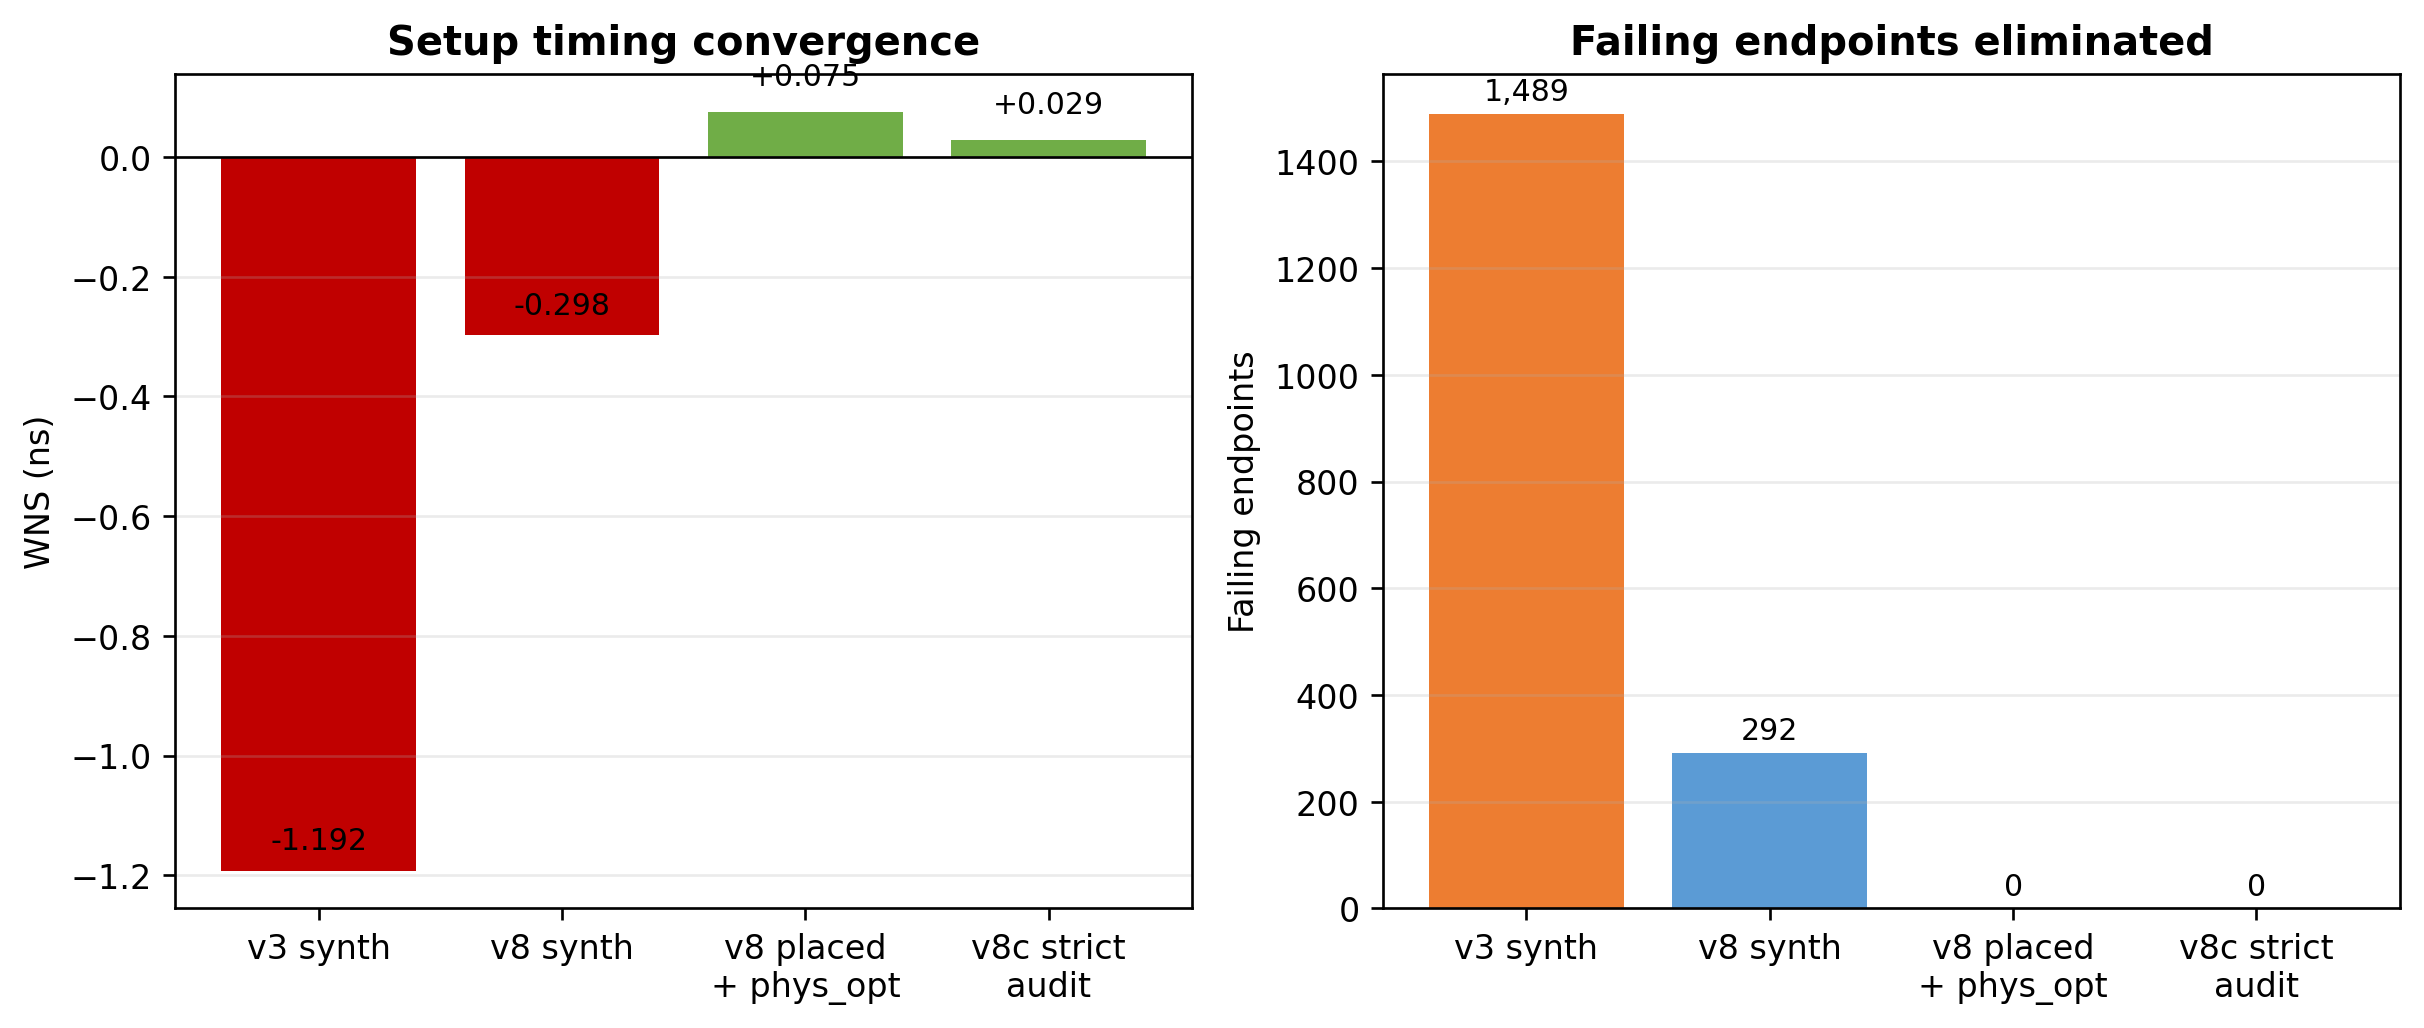
\includegraphics[width=\linewidth]{timing_iterations.png}
\caption{Board wrapper 從 wide registers 到 final route 的 timing 收斂}
\end{figure}

\begin{table}[H]
\centering
\caption{Timing iteration 詳細數據}
\begin{tabular}{lrrrrrr}
\toprule
Stage & WNS & TNS & Setup FEP & WHS & THS & Hold FEP \\
\midrule
v3 synthesis & $-1.192$ & $-1506.136$ & 1,489 & $+0.049$ & 0 & 0 \\
v8 synthesis & $-0.298$ & $-11.728$ & 292 & $+0.045$ & 0 & 0 \\
v8 placed + phys\_opt & $+0.075$ & 0 & 0 & $-0.082$ & $-0.364$ & 9 \\
Final v8c strict audit & $+0.029$ & 0 & 0 & $+0.044$ & 0 & 0 \\
\bottomrule
\end{tabular}
\end{table}

Synthesis 未通過並不表示最終一定失敗，因為其 interconnect estimate 尚未有真實 placement。Physical optimization 讓 setup 轉正，但 placement checkpoint 的 hold 仍有 9 個 failing endpoints；route 與 post-route physical optimization 加入實際 routing/hold repair 後，setup/hold 同時通過。Final strict audit 另確認 pulse-width WPWS $+1.607$ ns、TPWS 0、failing endpoints 0；timing report 明確顯示「All user specified timing constraints are met」。

\section{175 MHz final scope 與 throughput 補償}

本版 production target 固定為 175 MHz。為避免 clock target 調整後 throughput 低於 1 Gbit/s，設計以兩個 first-block engines 與兩筆 data queue 消除 startup stalls，以提高每個 clock 的有效工作比例。Final v8c strict audit 與六模式 throughput regression 分別驗證 timing 與 $>1$ Gbit/s 的 RTL payload throughput。

\section{Final route 與 DRC}

\begin{table}[H]
\centering
\caption{Route、DRC 與 methodology 摘要}
\begin{tabularx}{\linewidth}{l r X}
\toprule
檢查 & 結果 & 說明 \\
\midrule
Logical nets & 25,065 & 7,307 不需 routing；17,758 routable \\
Fully routed nets & 17,758 & 100\% \\
Routing errors & 0 & 無 failed/unrouted/overlap nets \\
DRC Error & 0 & Hard gate pass \\
DRC Critical Warning & 0 & Hard gate pass \\
Methodology Error / Critical Warning & 0 / 0 & 2 個一般 \code{SYNTH-6 Warning} \\
CDC & 2 safe / 0 unsafe & reset request 與 UART RX 皆為 depth-2 \code{ASYNC_REG} synchronizer \\
\code{check_timing} & 10 critical categories = 0 & async/status input/output false-path allowlists = 2 / 5 \\
Pulse width & WPWS $+1.607$ ns / TPWS 0 & failing endpoints 0 \\
\bottomrule
\end{tabularx}
\end{table}

\chapter{Wrapper、UART 封包與傳輸效率}

\section{AXI wrapper}

\code{aes_gcm_axi_top.v} 是主要 integration wrapper：

\begin{itemize}
  \item 32-bit AXI4-Lite register interface：寫入 key words、mode、IV/AAD/data/tag bit lengths、command；讀取 status。
  \item 8-bit AXI4-Stream input：依 descriptor 順序傳 IV、AAD、PT/CT 與 decrypt tag，使用 \code{TVALID/TREADY/TLAST}。
  \item 三個 8-bit AXI4-Stream outputs：data、tag、result status；data 的 \code{TUSER} 表示 result class。
\end{itemize}

它是手寫 RTL wrapper，目前 repository 沒有 \code{.xci}，也不是 Xilinx IP Integrator 自動產生的 packaged IP。若後續要放入 block design，可再建立 IP-XACT component packaging，但這不影響現在 RTL/board signoff。

\section{UART board wrapper}

\code{arty_a7_100t_aes_gcm_uart_rsp_top.v} 使用：

\begin{itemize}
  \item Xilinx \code{MMCME2\_BASE} 與 \code{BUFG} primitives 產生 175 MHz；
  \item \code{mmcm\_locked \&\& rst\_btn} 先進入 2-stage \code{ASYNC\_REG} synchronizer，再經 4-stage stable-high qualifier 產生 synchronous \code{aresetn}；
  \item 手寫 \code{uart\_rx.v} 與 \code{uart\_tx.v}，不是 Xilinx AXI UART IP；
  \item \code{aes\_gcm\_uart\_rsp\_bridge.v} 將 UART frames 轉成 AXI4-Lite writes 與 AXI4-Stream data；
  \item LED 顯示 heartbeat、busy、last pass、last fail/MMCM unlock。
\end{itemize}

Reset directed XSim test 拒絕 1--3 個 sampled clocks 的 button/LOCKED pulse 與 alternating chatter；continuous-valid input 在第 6 個 sampled edge 釋放 reset，invalid input 在第 3 個 sampled edge 讓 distributed reset 生效。Routed audit 另以結構 gate 確認 logical qualifier 有 4 stages；最後一階為了 physical fanout 複製成 4 個 cells，不是 4 個獨立邏輯 reset sources。CDC 報告的 2 條 async port path 使用 false path 並由 synchronizer 處理；downstream FF-to-FF stages 仍由 STA 檢查。

Host request frame 格式為
\begin{equation}
 \texttt{command[7:0]}\ \|\ \texttt{bit\_length[15:8]}\ \|\
 \texttt{bit\_length[7:0]}\ \|\ \texttt{payload}.
\end{equation}
Commands 為 MODE、KEY、IV、AAD、PT、CT、TAG、RUN；response frames 為 STATUS、DATA、TAG。Bridge 將 input payload 存於 8-bit distributed RAM，output data/tag 也先捕捉到 byte memories，再依 frame 回傳。這個 memory-based wrapper 是 board timing closure 的關鍵。

\section{Protocol efficiency 與錯誤處理}

UART 8N1 的 line coding efficiency 固定為 80\%；再乘上 $N/(N+3)$ 的 frame header efficiency。Bridge 檢查 key length、IV/AAD/data 最大 1024 bits、NIST tag lengths、busy state、AXI response、result watchdog 與 output length/TLAST/TUSER。錯誤以 BAD\_CFG、BUSY 或 AUTH\_FAIL 回應。Protocol simulation 已涵蓋 AES-128/192/256 encryption、decrypt success、decrypt auth-fail 與 data block，共 6/6 pass。

\chapter{Simulation、NIST 與 FPGA 實板驗證}

\section{RTL regressions}

Promotion 版本執行的主要驗證包括：

\begin{itemize}
  \item AXI smoke：7,676 cycles，PASS；
  \item throughput：六模式 16,820/17,039 cycles，全部 $>1$ Gbit/s；
  \item Round48、Round49、Round53 security/directed regressions；
  \item fast-zeroize 與 sensitive data-buffer clearing；
  \item NIST 525 與 NIST 5,255 suites；
  \item full NIST simulation：47,250/47,250，17,740,527 simulation cycles。
\end{itemize}

\section{UVM 與 formal 驗證邊界}

XSim 2021.1 的 UVM 1.2 constrained-random regression 使用 seeds 175001、175019 與 175039，每個 seed 8 個 scenarios，總計 scoreboard 24 checked、0 failed，UVM error/fatal 為 0/0，每個 seed 的維護中 functional coverage model 為 100.00\%。Coverage 包含 AES-128/192/256、encrypt/decrypt、96/non-96-bit IV、不同 AAD/data 長度與 valid/invalid authentication；這不是 code coverage、assertion coverage 或 exhaustive security coverage。本輪 evidence 另保存 15 個實際 compilation inputs 的 SHA-256，並把全域 UVM error/fatal counts 納入最終 PASS gate。

Yosys 0.33 SAT 完成 19 個 assumption-free combinational assertions：GHASH $T^{0\ldots16}$ 對 independent NIST one-bit shift reference 為 17/0，AES S-box 對 algebraic $GF(2^8)$ inverse/affine reference 與 injectivity為 2/0。這是 \textbf{partial formal PASS}，不包含 sequential GHASH control、FIFO/ZEROIZE temporal properties、whole AES-GCM equivalence、liveness、CDC、timing、power 或 side-channel proof，因此不宣稱 full formal closure。

\section{FPGA programming 狀態}

Vivado Hardware Manager 透過 target \code{Digilent/210319BE76DEA} 找到 \code{xc7a100t\_0}，\code{program\_board.tcl} 回報 \code{BOARD\_PROGRAM\_SUMMARY status=PASS}。程式化的 v8a bitstream SHA-256 為
\begin{center}
\hashpair{22791C17939C1BBC43539C35ABB19C31}{896425D26AA4721D5E4D4D3ACC5A686E}.
\end{center}
該 Tcl 會呼叫 \code{program\_hw\_devices} 與 \code{refresh\_hw\_device}，但不產生 configuration-memory readback attestation；因此本報告不額外宣稱 EOS/DONE/CRC 狀態。後續六模式 UART smoke 的 summary 全部綁定同一 bitstream hash，為板上 operational evidence。

Final strict audit v8c 另輸出 SHA-256 為 \code{DC951AAE0D388DA54836AD5950CA87CB8EEE4A94E5E7EFBB1A685439F0934942} 的 \code{.bit}；它的 bit-header SHA 與板測 v8a \code{.bit} 不同，所以本報告不宣稱 v8c \code{.bit} 曾被程式化。兩者的 raw configuration \code{.bin} SHA-256 則同為 \code{8A19D8E5900063B64922DC9B9AD323F953386367CA1D4FA1A61935543B4332F3}；這是 static-audit output 與 hardware-tested configuration 之間的 exact binary identity boundary。

\section{六模式 smoke 與 47,250 筆 NIST RSP final result}

\begin{table}[H]
\centering
\caption{FPGA hardware verification final status}
\begin{tabularx}{\linewidth}{l r r X}
\toprule
Test & Executed & Fail & Status / evidence \\
\midrule
AES-128 encrypt smoke & 1 & 0 & \pass; exact v8a bit hash \\
AES-192 encrypt smoke & 1 & 0 & \pass; exact v8a bit hash \\
AES-256 encrypt smoke & 1 & 0 & \pass; exact v8a bit hash \\
AES-128 decrypt smoke & 1 & 0 & \pass; exact v8a bit hash \\
AES-192 decrypt smoke & 1 & 0 & \pass; exact v8a bit hash \\
AES-256 decrypt smoke & 1 & 0 & \pass; exact v8a bit hash \\
Full NIST GCM RSP & 47,250 & 0 & \pass；47,250/47,250，first failure null \\
\bottomrule
\end{tabularx}
\end{table}

實板 runner 使用 COM4、115200 baud，逐筆比對 status、ciphertext/plaintext 與 authentication tag；decrypt FAIL vectors 必須回傳 AUTH\_FAIL 且不釋放 plaintext。Final summary 為 \code{requested=executed=pass=47250}、\code{fail=0}、\code{first\_failure=null}。JSONL 恰有 47,250 行、global indices 0--47,249 連續且唯一；六個 RSP source 各 7,875 筆。分類為 encrypt 23,625、decrypt 23,625，其中 decrypt success 11,717、expected authentication failure 11,908。Status/data/tag mismatch 均為 0，且第二位獨立 reconciliation 亦通過。

Host-observed per-case latency 的 min/mean/median/p95/p99/max 分別為 9.101/25.376/31.440/32.289/47.797/49.779 ms；全量 elapsed time 為 1,208.505 s，平均 39.098 cases/s。這組 latency 包含 UART 與 host transaction overhead，只能解讀為 board-validation harness 表現。

\begin{figure}[H]
\centering
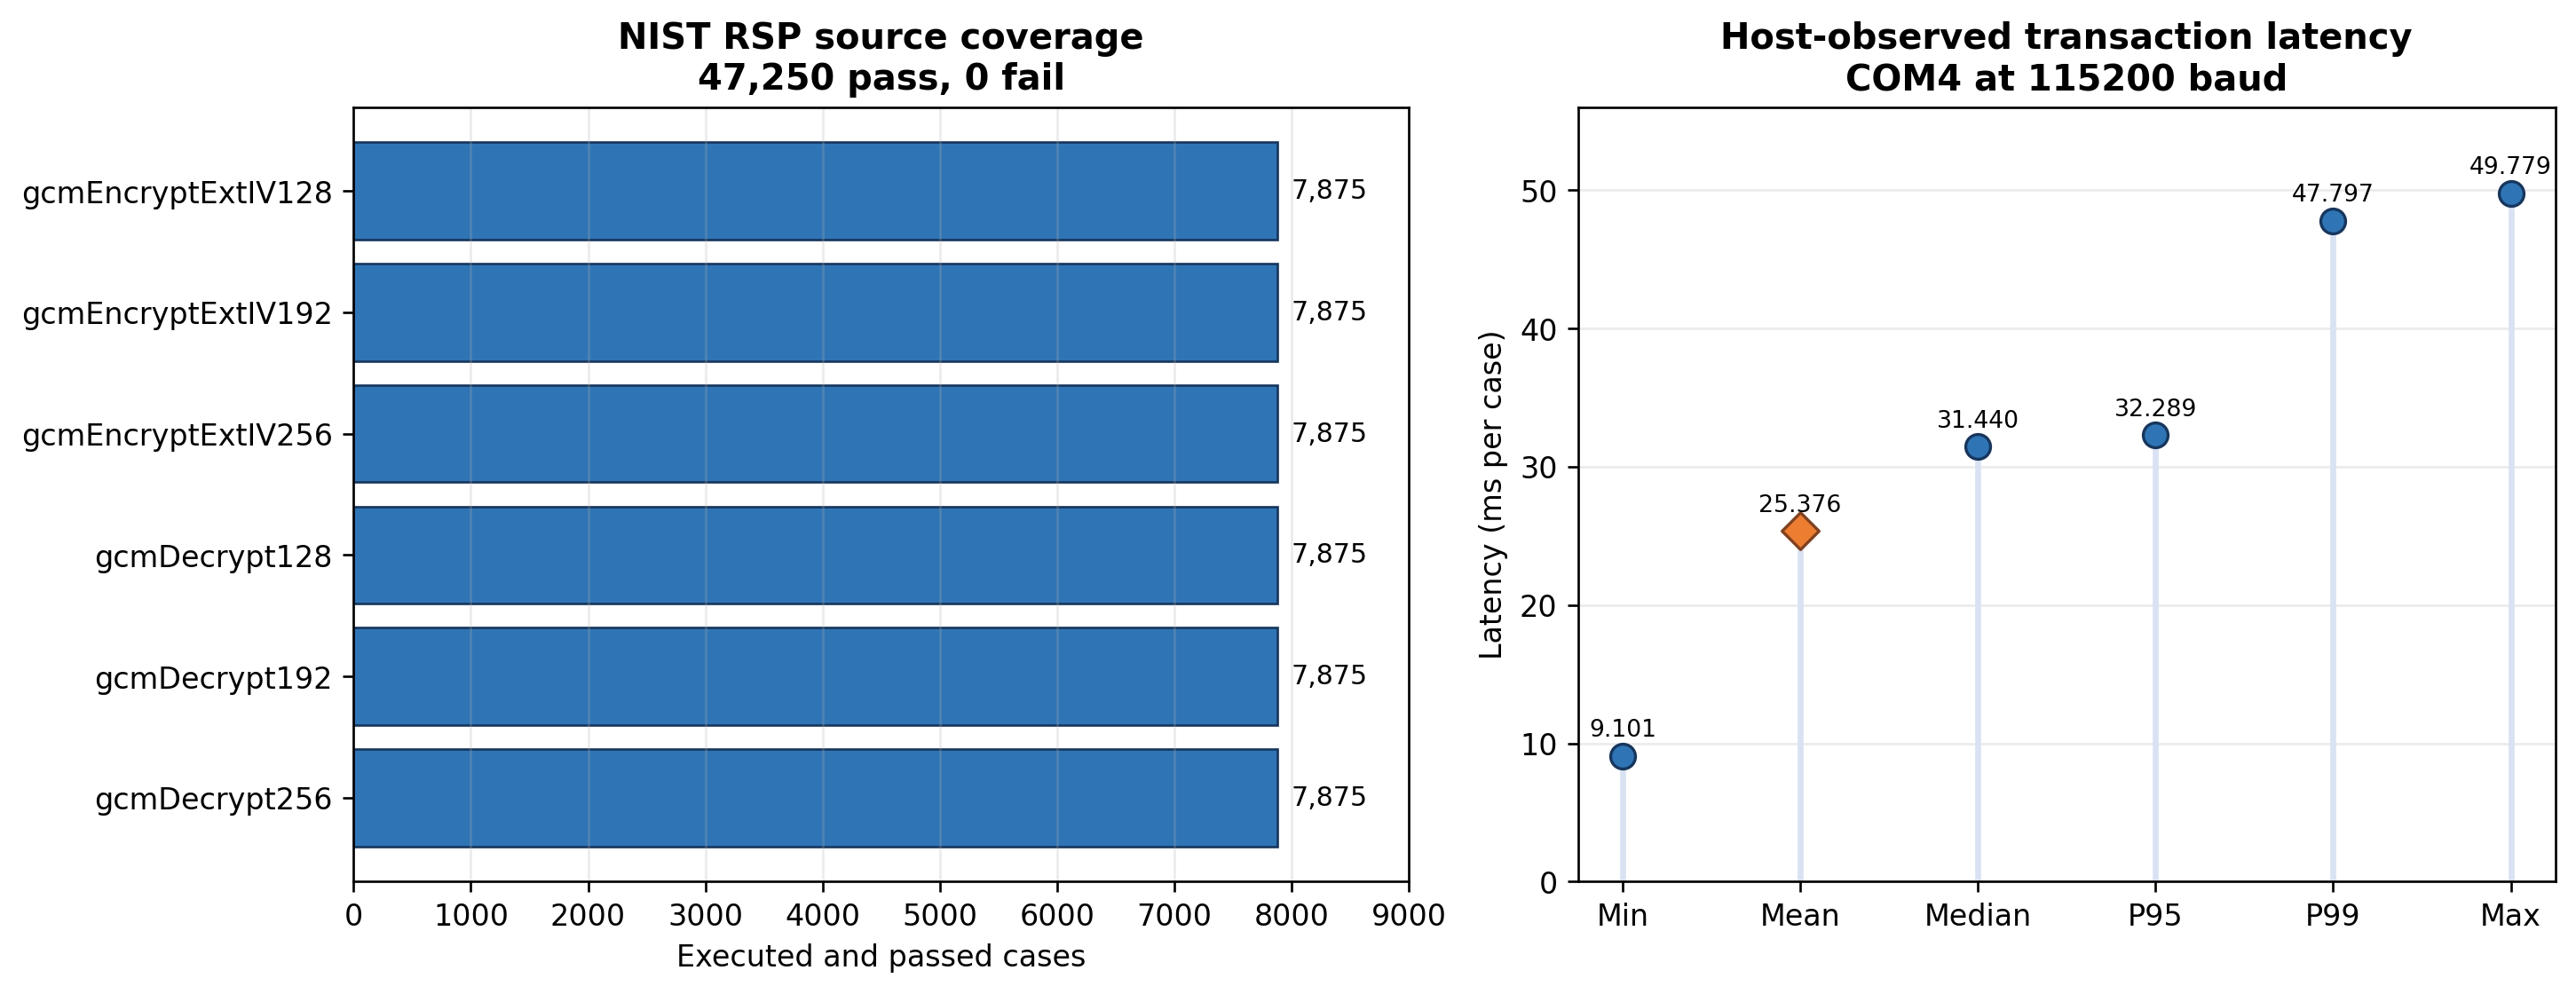
\includegraphics[width=\linewidth]{nist_validation.png}
\caption{Full FPGA NIST source coverage 與 host-observed latency。左圖六個 RSP source 各執行並通過 7,875 筆；右圖呈現 min、mean、median、p95、p99 與 max。這不是 AES-GCM core cycle latency。}
\end{figure}

\chapter{遇到的問題、根因與解法}

\begin{longtable}{p{0.20\linewidth}p{0.28\linewidth}p{0.42\linewidth}}
\caption{主要問題與處置}\label{tab:issues}\\
\toprule
問題 & 根因 & 解法與結果 \\
\midrule
\endfirsthead
\toprule
問題 & 根因 & 解法與結果 \\
\midrule
\endhead
175 MHz 原架構 throughput 不足 1 Gbit/s & 每筆 record 最前面的 AES keystream latency 造成 byte-stream bubble & 增加兩個 specialized first-block engines、16-entry keystream FIFO 配合兩筆 sensitive data queue；達 1.065/1.052 Gbit/s \\
\addlinespace
Board v3 synth WNS $-1.192$ ns、TNS $-1506.136$ ns & UART bridge 的 1024-bit payload 被實作為 FF arrays，dynamic indexed write/capture 形成大 mux 與高 fanout & 改為 8-bit distributed memories；LUT/FF 大幅下降，synth TNS 改善到 $-11.728$ ns \\
\addlinespace
Protocol simulation stream byte 不前進 & combinational helper function 直接讀 global registers，XSIM 沒有依預期重新評估資料依賴 & 改為直接 combinational expression，6/6 protocol cases pass \\
\addlinespace
Placed setup pass 但 hold fail & Physical optimization 改善 setup 後產生 9 個 short-path hold violations & Explore route 與 post-route hold repair 後 WHS $+0.044$ ns、THS 0 \\
\addlinespace
功率數字可信度有限 & 無真實 SAIF/VCD，Vivado vectorless 使用預設 activity propagation & 報告只列 0.461 W Medium-confidence estimate；下一步加入 representative workload SAIF 或量測板級 rails \\
\addlinespace
Asynchronous run request 可造成錯誤 reset release & 單純 shift chain 會把短 pulse 延遲成一個有效 release sample & 分離 2-stage \code{ASYNC\_REG} synchronizer 與 4-stage stable-high qualifier；directed XSim、CDC schema 與 routed structural gate 通過 \\
\addlinespace
UART 無法顯示 1 Gbit/s & 115200 baud 物理限制，8N1 payload ceiling 92.16 kbit/s & 清楚區分 core throughput 與 board transport；若要板上高速量測需換 DMA/Ethernet/PCIe 或 on-chip counter \\
\bottomrule
\end{longtable}

\chapter{工具、Tcl 驅動方式與檔案位置}

\section{本次使用的工具}

\begin{table}[H]
\centering
\caption{工具與用途}
\begin{tabularx}{\linewidth}{l l X}
\toprule
工具 & 版本 / 介面 & 用途 \\
\midrule
Vivado & 2021.1 build 3247384 & synth、opt、place、phys\_opt、route、timing、utilization、power、DRC、bitgen、Hardware Manager \\
XSIM & Vivado 2021.1 & smoke、throughput、security regressions、NIST simulation、UART protocol simulation \\
UVM 1.2 & XSim 2021.1 & 3 seeds、24 scenarios、scoreboard 與 functional coverage \\
Yosys SAT & 0.33 & GHASH shift transform 與 AES S-box 的 19 個 combinational assertions \\
Tcl & Vivado Tcl shell & 可重現 flow、DCP hash gate、reports 與 hard gates \\
PowerShell & Windows & 啟動 batch flow、整理驗證輸出與環境檢查 \\
Python + pyserial & Host COM4 & parse NIST \code{.rsp}、送 UART frames、比對結果、輸出 JSONL evidence \\
\code{Get-FileHash} & PowerShell & SHA-256 DCP/bitstream/evidence identity \\
Git & branch/commit & 保存 RTL、tests、Tcl 與可追溯變更 \\
LaTeX/Tectonic & XeTeX-compatible & 產生本報告 PDF \\
\bottomrule
\end{tabularx}
\end{table}

「OpenShell」不是此專案的必要工具。這次主要使用 PowerShell 呼叫 Vivado batch Tcl；Vivado 自身也有 Tcl console。GUI 只用於 Hardware Manager/JTAG programming 與需要時的 interactive Device view。

\section{如何驅動 Tcl}

Fresh board build：
\begin{lstlisting}[language=bash]
C:\Xilinx\Vivado\2021.1\bin\vivado.bat -mode batch \
  -source C:\project\FPGA3\engrenring\synth_1g\board\run_arty_a7_100t_uart_rsp.tcl \
  -tclargs <unique_output_directory>
\end{lstlisting}

從 verified synth DCP resume：
\begin{lstlisting}[language=bash]
C:\Xilinx\Vivado\2021.1\bin\vivado.bat -mode batch \
  -source C:\project\FPGA3\engrenring\synth_1g\board\run_arty_a7_100t_uart_rsp_from_synth.tcl \
  -tclargs <synth.dcp> <expected_sha256> <unique_output_directory>
\end{lstlisting}

Host NIST RSP runner：
\begin{lstlisting}[language=bash]
python C:\project\FPGA3\engrenring\synth_1g\board\run_nist_rsp_uart.py \
  --port COM4 --baud 115200 --stop-on-fail \
  --bitstream <final.bit> --output <evidence.jsonl> <six_rsp_files>
\end{lstlisting}

\section{RTL 與 wrapper 位置}

\begin{longtable}{p{0.27\linewidth}p{0.65\linewidth}}
\caption{主要 RTL 檔案}\label{tab:rtl-files}\\
\toprule
功能 & 絕對路徑 \\
\midrule
\endfirsthead
\toprule
功能 & 絕對路徑 \\
\midrule
\endhead
AXI top wrapper & \path{C:/project/FPGA3/engrenring/rtl/source/aes_gcm_axi_top.v} \\
AES-GCM stream core & \path{C:/project/FPGA3/engrenring/rtl/source/stream_core/aes_gcm_stream_core.v} \\
Main AES engine & \path{C:/project/FPGA3/engrenring/rtl/source/stream_aes/aes_block_engine.v} \\
First-block AES engine & \path{C:/project/FPGA3/engrenring/rtl/source/stream_aes/aes_first_block_engine.v} \\
Key expansion & \path{C:/project/FPGA3/engrenring/rtl/source/stream_aes/aes_key_context.v} \\
AES S-box & \path{C:/project/FPGA3/engrenring/rtl/source/aes_core/sbox.v} \\
GHASH16 & \path{C:/project/FPGA3/engrenring/rtl/source/stream_ghash/ghash16.v} \\
Generic FIFO & \path{C:/project/FPGA3/engrenring/rtl/source/stream_core/stream_fifo.v} \\
AXI-Lite registers & \path{C:/project/FPGA3/engrenring/rtl/source/stream_axi/axi_lite_regs.v} \\
UART board top & \path{C:/project/FPGA3/engrenring/rtl/source/board/arty_a7_100t_aes_gcm_uart_rsp_top.v} \\
UART RSP bridge & \path{C:/project/FPGA3/engrenring/rtl/source/board/aes_gcm_uart_rsp_bridge.v} \\
UART RX/TX & \path{C:/project/FPGA3/engrenring/rtl/source/board/uart_rx.v}、\path{uart_tx.v} \\
\bottomrule
\end{longtable}

\section{Final implementation、圖片與證據位置}

Final strict static-audit evidence directory：
\begin{center}
\small\path{C:/project/FPGA3/engrenring/synth_1g/board/output/ece78ce_uart_rsp_175_resetqual4_audit_v8c}
\end{center}
Hardware programming、smoke 與 NIST evidence directory 為
\begin{center}
\small\path{C:/project/FPGA3/engrenring/synth_1g/board/output/ece78ce_uart_rsp_175_resetqual4_audit_v8a}.
\end{center}
其 immutable synth/placed/routed DCP 來源目錄為
\begin{center}
\small\path{C:/project/FPGA3/engrenring/synth_1g/board/output/ece78ce_uart_rsp_175_resetqual4_final_v8}.
\end{center}

其中重要檔案如下：

\begin{longtable}{p{0.29\linewidth}p{0.63\linewidth}}
\toprule
檔案 & 用途 \\
\midrule
\endfirsthead
\toprule
檔案 & 用途 \\
\midrule
\endhead
v8c \path{arty_a7_100t_aes_gcm_uart_rsp_top.bit}、\path{arty_a7_100t_aes_gcm_uart_rsp_top.bin} & strict-audit outputs；\code{.bin} 與 hardware-tested v8a config image exact match \\
v8a \path{arty_a7_100t_aes_gcm_uart_rsp_top.bit} & Hardware Manager 實際程式化，且由 smoke/NIST exact hash 綁定的 bitstream \\
v8 \path{*_synth.dcp}、\path{*_placed.dcp}、\path{*_routed.dcp} & fresh build checkpoints；routed DCP 是 v8c strict audit 的 hash-gated input \\
v8c \path{signoff_metrics.txt} & routed DCP identity、setup/hold/pulse-width、route/CDC/reset/check\_timing hard-gate summary \\
v8c \path{timing_routed.rpt} & WNS/TNS/WHS/THS/WPWS/TPWS 與 critical paths \\
v8c \path{utilization_routed.rpt} & LUT/FF/LUTRAM/BRAM hierarchy \\
v8c \path{route_status.rpt} & fully routed nets 與 routing error \\
v8c \path{drc_routed.rpt}、\path{methodology_routed.rpt} & DRC 0；methodology E/CW 0 與 2 個一般 warnings \\
v8c \path{cdc_routed.rpt}、\path{check_timing_routed.rpt} & synchronizer schema 與 exact false-path allowlists \\
v8c \path{power_vectorless_routed.rpt} & 0.461 W Medium-confidence vectorless estimate \\
v8c \path{clock_utilization_routed.rpt} & MMCM/BUFG、clock loads 與 clock regions \\
v8a \path{program_board.log} & Hardware Manager programming terminal evidence \\
v8a \path{hw_smoke_*.jsonl}、\path{hw_smoke_*.summary.json} & AES-128/192/256 encrypt/decrypt 六模式，6/0 \\
v8a \path{hw_nist_47250.jsonl} & 47,250 行逐向量 evidence；indices/source/classification/status-data-tag reconciliation 全通過 \\
v8a \path{hw_nist_47250.summary.json}、\path{hw_nist_47250_run.log} & 47,250/47,250、fail 0、first failure null、elapsed 1,208.505 s \\
\bottomrule
\end{longtable}

本報告的圖檔在：
\begin{center}
\small\path{C:/project/FPGA3/docs/report/figures}
\end{center}
可由 \path{C:/project/FPGA3/docs/report/generate_figures.py} 重新產生。

\chapter{結論與後續工作}

本版已完成可燒錄的 Arty A7-100T AES-GCM 實作，175 MHz v8c strict static audit 的 setup、hold、pulse-width、route、DRC、methodology E/CW、CDC/reset schema 與 \code{check\_timing} hard gates 全部通過。Hardware-tested v8a bitstream 的 configuration \code{.bin} 與 v8c strict-audit \code{.bin} 完全相同；其六模式 smoke 為 6/0，full hardware NIST 為 47,250/47,250、fail 0，且第二位獨立 reconciliation 通過。核心透過兩個 first-block engines、三 context shared AES pipeline、16-entry keystream FIFO、兩筆 sensitive data queue 與 16-bit digit-serial GHASH，在單一 8-bit stream 下達到 1.065398 Gbit/s encryption 與 1.051705 Gbit/s decryption。

Standalone OOC PartPin 狀態仍為 \textbf{NO / NOT RUN}：目前沒有 approved、identity-matched production \code{HD.PARTPIN\_LOCS} map 與 parent timing model。此限制與已通過的 full-board route 是不同 signoff boundary。

下一步建議依風險排序：

\begin{enumerate}
  \item 封存 v8c strict-audit 與 v8a board evidence 的 manifest、SHA-256 與 reconciliation 規則；未來重跑必須先核對 routed DCP 與 configuration image identity。
  \item 以代表性 SAIF/VCD 重跑 power，或量測 FPGA 電源 rails，替換 Medium-confidence vectorless 數字。
  \item 擴充 sequential formal adapter/solver，覆蓋 GHASH control、FIFO/ZEROIZE temporal behavior 與 top-level liveness；不把 19 個 combinational assertions 誤當 full closure。
  \item 若交付範圍需要 PartPin，先取得 approved identity-matched production map 與 parent timing model，再執行 strict replay。
  \item 若要證明板上 crypto datapath 的 1 Gbit/s，而不只是 simulation，加入 on-chip cycle counter + BRAM traffic generator，或改用 Ethernet/PCIe/高速 AXI DMA。
  \item 若要正式交付 Vivado Block Design，將 \code{aes_gcm_axi_top} 另行 package 成 IP-XACT，並建立 CDC、register-map 與 driver 文件。
\end{enumerate}

\appendix
\chapter{Artifact identity 與 hashes}

\begin{table}[H]
\centering
\caption{Final artifact SHA-256}
\begin{tabularx}{\linewidth}{l X}
\toprule
Artifact & SHA-256 \\
\midrule
v8 synth DCP & \hashpair{C5D9858BDD097622C7AA76A1843CB3D4}{9EF7646470BC4ACDAF9BDB27882914E6} \\
v8 placed DCP & \hashpair{82BAA9B402F825B3127202255F5787BA}{82A8E7F34291A0DDA5F4C86689C4119D} \\
v8 routed DCP / v8c strict-audit input & \hashpair{A91758ED87EB56648EEF0CAB67B2C50D}{198D00A2D5088E624B507687D99C016B} \\
v8c audit script & \hashpair{62C653E5E49723A51726B92B0D475BA1}{1C55F24A3648D59359A2ABCE99C9286E} \\
v8c bitstream & \hashpair{DC951AAE0D388DA54836AD5950CA87CB}{8EEE4A94E5E7EFBB1A685439F0934942} \\
v8c binary / hardware-tested v8a binary & \hashpair{8A19D8E5900063B64922DC9B9AD323F9}{53386367CA1D4FA1A61935543B4332F3} \\
Hardware-tested v8a bitstream & \hashpair{22791C17939C1BBC43539C35ABB19C31}{896425D26AA4721D5E4D4D3ACC5A686E} \\
v8c signoff metrics & \hashpair{CBC7D4F16D9D54A67CC6B10E4A9DC612}{888112933D6263F3F2D69932FB0946CB} \\
v8c routed power report & \hashpair{687014688995046BACE3FFA09CB4E3E3}{B76A551B0F9A1D3C92C7C6874A9EF351} \\
UVM summary CSV & \hashpair{F46216BF196C08ED466200EE34E3F2A7}{B626EB376E7C0F8A758DCB47B3225641} \\
UVM summary JSON & \hashpair{F5B8E59504D967B6841AD73E0B6E3D8}{361162E251CF7FED2F303682C8B8500AF} \\
UVM compile-input manifest & \hashpair{D36DA381A5326EEBB1DABDA4AD63D45}{421ACE5E433CE38A3EF80494002233292} \\
Formal run log & \hashpair{C1FB4DA19869532E1831069A635BF71F}{7C6714237DD5C08C7EDF6A16CCBC0C96} \\
NIST FPGA JSONL & \hashpair{56DA5E1B7110AE8A5622B5847211A842}{C4D2A2A22A08EE02AA7D32EFB0C59761} \\
NIST FPGA summary & \hashpair{5DF2EA729BBD0C19C6677AFD13F73DD4}{F04BB53694B9552A3FF4D9D464604D06} \\
NIST FPGA run log & \hashpair{B861E8500B214CB85A98A1FDC231C3E0}{97DDA60F237EA3A49021E6BCECEFEEB4} \\
\bottomrule
\end{tabularx}
\end{table}

\chapter{參考資料}

\begin{thebibliography}{99}
\bibitem{fips197}
National Institute of Standards and Technology, \emph{Advanced Encryption Standard (AES)}, FIPS PUB 197, 2001. Local file: \path{reference/[02] NIST_FIPS_197_AES.pdf}.

\bibitem{sp80038d}
Morris Dworkin, \emph{Recommendation for Block Cipher Modes of Operation: Galois/Counter Mode (GCM) and GMAC}, NIST SP 800-38D, 2007. Local file: \path{reference/[03] NIST_SP_800-38D_GCM_GMAC.pdf}.

\bibitem{satohgcm}
Akashi Satoh, ``High-Speed Hardware Architectures for Authenticated Encryption Mode GCM,'' ISCAS, 2006. Local file: \path{reference/[08] Satoh_High-Speed_GCM_Hardware_Architectures.pdf}.

\bibitem{henzen}
Luca Henzen and Wolfgang Fichtner, ``FPGA Parallel-Pipelined AES-GCM Core for 100G Ethernet Applications,'' 2010. Local file: \path{reference/[09] Henzen_Fichtner_FPGA_Parallel_Pipelined_AES-GCM_100G.pdf}.

\bibitem{joshi}
Arundhati Joshi, P. K. Dakhole, and Ajay Thatere, ``Implementation of S-Box for Advanced Encryption Standard,'' ICETECH, 2015. Local file: \path{reference/[17] Joshi_Implementation_of_S-Box_for_AES.pdf}.

\bibitem{zhangparhi}
Xinmiao Zhang and Keshab K. Parhi, ``High-Speed VLSI Architectures for the AES Algorithm,'' IEEE Transactions on VLSI Systems, vol. 12, no. 9, 2004. Local file: \path{reference/[18] Zhang_Parhi_High-Speed_VLSI_AES.pdf}.

\bibitem{satohcompact}
Akashi Satoh, Sumio Morioka, Kohji Takano, and Seiji Munetoh, ``A Compact Rijndael Hardware Architecture with S-Box Optimization,'' ASIACRYPT, 2001. Local file: \path{reference/[20] Satoh_Compact_Rijndael_Hardware_Architecture.pdf}.

\bibitem{zhoukoa}
Gang Zhou, Harald Michalik, and L\'aszl\'o Hinsenkamp, ``Improving Throughput of AES-GCM with Pipelined Karatsuba Multipliers on FPGAs,'' ARC, 2009. Local file: \path{reference/[28] Zhou_Pipelined_Karatsuba_AES-GCM_FPGA.pdf}.
\end{thebibliography}

\end{document}
